% !TeX program = pdflatex
% !TeX encoding = UTF-8
% !TeX spellcheck = pt_BR
\documentclass[
  article,
  11pt,
  a4paper,
  english,
  brazil,
  sumario=tradicional]{abntex2}
\usepackage{lmodern}			% Usa a fonte Latin Modern
\usepackage[T1]{fontenc}		% Seleção de códigos de fonte.
\usepackage[utf8]{inputenc}		% Codificação do documento (conversão automática dos acentos)
\usepackage{indentfirst}		% Indenta o primeiro parágrafo de cada seção.
\usepackage{nomencl} 			% Lista de simbolos
\usepackage{color}				% Controle das cores
\usepackage{graphicx}			% Inclusão de gráficos
\usepackage{microtype} 			% Melhorias de justificação
\usepackage{csquotes}			% Aspas e citações mais simples
\usepackage{booktabs}			% Tabelas mais profissionais

% ---
% Pacotes de citações
% ---
\usepackage[brazilian,hyperpageref]{backref}	 % Paginas com as citações na bibliografia
\usepackage[alf]{abntex2cite}	% Citações padrão ABNT
% ---

% ---
% Configurações do pacote backref
% Usado sem a opção hyperpageref de backref
\renewcommand{\backrefpagesname}{Citado na(s) página(s):~}
% Texto padrão antes do número das páginas
\renewcommand{\backref}{}
% Define os textos da citação
\renewcommand*{\backrefalt}[4]{
  \ifcase #1 %
  Nenhuma citação no texto.%
  \or
  Citado na página #2.%
  \else
  Citado #1 vezes nas páginas #2.%
  \fi}%
% ---

% Para fórmulas matemáticas
\usepackage{amsmath}
\usepackage{amssymb}
\usepackage{mathtools}

% Para setas usadas em fórmulas dos grafos
\usepackage{MnSymbol}

% Diretório padrão para figuras
\graphicspath{ {images/} }

% Permite colocar figuras lado a lado ou
% fazer posicionamentos arbitrários
\usepackage[lofdepth,lotdepth]{subfig}

\hypersetup{
  %hidelinks,   % Comente aqui para exibir os links
  colorlinks, % Descomente esse se comentar o de cima
  linkcolor={red!50!black},
  citecolor={blue!50!black},
  urlcolor={blue!80!black}
}

\usepackage[pdftex,dvipsnames,table,xcdraw]{xcolor}

% ---
% Altera as margens padrões
% ---
\setlrmarginsandblock{3cm}{3cm}{*}
\setulmarginsandblock{3cm}{3cm}{*}
\checkandfixthelayout
% ---

% --- 
% Espaçamentos entre linhas e parágrafos 
% --- 

% O tamanho do parágrafo é dado por:
\setlength{\parindent}{1.3cm}

% Controle do espaçamento entre um parágrafo e outro:
\setlength{\parskip}{0.2cm}  % tente também \onelineskip

% Espaçamento simples
\SingleSpacing

% Titulo e coisas para cabeçalho
\title{Compressão de Fluxo para Identificação de Fronteiras de Carreiras}
\author{Ronie Uliana and Leandro Nunes de Castro}

\begin{document}

% Seleciona o idioma do documento (conforme pacotes do babel)
%\selectlanguage{english}
\selectlanguage{brazil}

% Retira espaço extra obsoleto entre as frases.
\frenchspacing

\maketitle

\begin{abstract}
Resumo vai aqui
\end{abstract}

%===================================
\section{Introdução}
%===================================

Cada trajetória profissional é bastante particular. Enquanto alguns seguem caminhos bem definidos, como inúmeros presidentes de empresas que começaram como estagiários, outros trilham por sequências improváveis de ocupações, como o início da carreira de Sílvio Santos, que foi Camelô e Paraquedista Militar antes de começar a carreira como Apresentador de TV; ou Monja Coen, que foi jornalista até seus 36 anos antes de se tornar uma Monja Budista.

Também os modelos de carreiras têm se modificado e teorias como as das \textit{Carreiras Proteanas} e \textit{Carreiras sem Fronteiras} advogam um distanciamento das carreiras comuns em favor de trajetórias com foco maior no indivíduo~\cite{Bendassolli2009-bg}. A carreira proteana coloca o indivíduo, e não as organizações, como protagonista da trajetória profissional, onde seus valores são usados na decisão dos próximos passos e o sucesso é subjetivo e medido pela satisfação pessoal~\cite{Hall2004-ke}. A carreira sem fronteiras, por sua vez, acontece quando a trajetória se faz independente das organizações ou hierarquias. Essas carreiras são caracterizadas por passagens por múltiplas empresas ou mudanças na especialidade do indivíduo, como um eletricista industrial que passa a atuar como web designer~\cite{Arthur1994-qq}.

No entanto, o movimento de uma pessoa entre ocupações profissionais não é simples. A capacitação do indivíduo, a atratividade da nova ocupação e o próprio conhecimento de que uma transição é possível a tornam mais fácil ou difícil para os profissionais. Quando essa transição é percebida como uma barreira por um número suficiente de pessoas, surge uma \textit{fronteira de carreira}~\cite{Gunz2007-hr}. Essas fronteiras delimitam um grupo de ocupações nas quais um indivíduo tem maiores chances de permanecer durante sua trajetória profissional, denominado aqui como \textit{ilha ocupacional}.

Esse trabalho utiliza o conceito de fronteira de carreira~\cite{Gunz2007-hr}, um banco de dados com milhões de experiências profissionais ~\cite{VAGAS_Tecnologia2014-yv} e técnicas de detecção de comunidades em redes~\cite{Rosvall2009-sd,Edler2017-kt} para encontrar ilhas ocupacionais no mercado de trabalho brasileiro, discutir e entender sua estrutura.

O estudo revela onde estão as fronteiras das ilhas, quais suas composições e apresenta \textit{insights} sobre suas estruturas. O resultado obtido pode ser usado para o refinamento de teorias sobre carreira, como uma classificação natural para as ocupações baseada na movimentação profissional ou como subsídio para o planejamento de carreiras.

A principal contribuição desse trabalho está em tornar concreto o conceito de \textit{fronteiras de carreira}, aplicando técnicas de Ciência de Redes para revelar a estrutura da movimentação profissional no Brasil. O trabalho se estende nesse processo, derivando o conceito de ilha ocupacional a partir das fronteiras de carreiras como grupos de ocupação que se isolam de outros, onde a movimentação inter-ilhas é rara em comparação à movimentação intra-ilhas.

Explorando esse conceito, o trabalho caracteriza a topologia das ilhas ocupacionais e propõe a identificação de \textit{polos ocupacionais} como ocupações que possuem papel crucial na estrutura. A topologia encontrada na maior parte das ilhas tende a um formato estrelado, sugerindo que a atuação nos polos afeta a ilha como um todo.

A presença de uma ilha gigante nos resultados fornece indícios que suportam o modelo de \textit{Carreira sem Fronteiras}, ao mesmo tempo em que indica que ela não abrange todos os segmentos profissionais.

Esse artigo está organizado da seguinte forma. A Seção~\ref{sec:carreira} descreve o conceito de fronteira da carreira, enquanto a Seção~\ref{sec:mapa} descreve o banco de dados utilizado na pesquisa. As Seções~\ref{sec:comunidades} e~\ref{sec:assortatividade} descrevem os algoritmos empregados para detecção de comunidades e a medição utilizada na caracterização da topologia. Finalmente, a Seção~\ref{sec:resultados} discute e levanta questões sobre os resultados obtidos.

%===================================
\section{Sobre Carreira e seus Conceitos Associados} \label{sec:carreira}
%===================================

Segundo~\citeonline{Arthur1989-rn}, carreira é \foreignquote{english}{uma sequência evolutiva da experiência profissional de uma pessoa no tempo}\footnote{No original: \enquote{an evolving sequence of person's work experience over time}.}.

Apesar das discussões sobre as mudanças nos modelos de carreira, passando de um modelo linear e centrado na organização para um modelo centrado no indivíduo, as definições de carreira são frequentemente associadas à progressão profissional do indivíduo~\cite{Baruch2004-oy,Sullivan2009-xb,Bendassolli2009-bg}.

Para os fins desse trabalho, define-se carreira como \textit{a sequência de \textbf{ocupações} pela qual um indivíduo passa em sua vida profissional}. Essa definição é similar à de \citeonline{Arthur1989-rn}, porém, limita sua abrangência e a torna mais concreta. Isso permite uma análise menos subjetiva, uma vez que ocupações profissionais podem ser extraídas de currículos e analisadas quantitativamente. No entanto, ela se torna mais limitada, já que essa definição exclui aspectos psicológicos ou sociais.

Essa pesquisa empresta o conceito de \textit{fronteiras de carreira} (\textit{career boundaries}) descrito por \citeonline{Gunz2007-hr} para dar significado ao trabalho. A fronteira de carreira significa que uma mudança entre ocupações nem sempre pode ser realizada livremente. Por exemplo, um profissional precisa de graduação especializada antes de poder se mover da ocupação de \enquote{Auxiliar de Jardinagem} para \enquote{Médico}, por outro lado, a barreira para o mesmo profissional exercer a ocupação de \enquote{Jardineiro} se limita à experiência. É possível perceber que as barreiras não são simétricas, em tempos de crise econômica é mais simples para um \enquote{Engenheiro} tornar-se um \enquote{Corretor de Imóveis} do que o contrário.

As barreiras não se limitam ao conhecimento, quaisquer dificuldades na movimentação podem criar fronteiras. Por exemplo, alguém morando em um grande centro urbano dificilmente exerceria a ocupação de \enquote{Agricultor} sem mover-se para o campo. Um \enquote{Diretor Financeiro} precisaria adequar seu padrão de vida antes de uma transição para uma ocupação com ganhos mais modestos. Uma profissão que está desaparecendo, como \enquote{Contínuo}, possui barreiras mais altas do que uma nascendo, como \enquote{Analista de Experiência do Usuário}.

Um dos pontos principais desse trabalho está na argumentação de \citeonline{Gunz2007-hr} sobre como uma fronteira subjetiva se torna objetiva. Em sua argumentação as fronteiras de carreira são subjetivas e pessoais, onde cada um tem para si quais transições podem ser feitas em sua própria carreira. No entanto, elas se tornam objetivas quando um número suficientemente grande de pessoas possui a mesma compreensão sobre essas transições, a ponto dela ser perceptível em um nível macroscópico.

Dessa maneira, as fronteiras de carreira são definidas objetivamente quando uma quantidade suficiente de pessoas entra em \textit{consenso} sobre quais são as transições incomuns.

Partindo desse pressuposto, a identificação de trajetórias comuns e incomuns é condição suficiente e necessária para a detecção de fronteiras entre carreiras. Suficiente, pois a própria definição de fronteira é dependente da identificação do que são transições \enquote{incomuns}. Necessária, pois não existem fronteiras objetivamente definidas sem o consenso.

Essas fronteiras isolam algumas ocupações das outras, criando um grupo coeso pelo distanciamento dos outros grupos e não por alguma característica intrínseca.  Ou seja, a fronteira define o grupo, e não o contrário~\cite{Gunz2007-hr,Abbott1995-ft}. 

No presente trabalho esses aglomerados de ocupações são chamados \textit{ilhas de ocupações} ou \textit{ilhas ocupacionais}, refletindo a facilidade de movimentação dentro de suas fronteiras e o distanciamento de outros grupos.

Como será visto a seguir, as ocupações serão representadas por nós em um grafo, enquanto as conexões trarão informações sobre as transições entre ocupações. Neste tipo de representação, outro conceito central introduzido para o desenvolvimento da pesquisa é o de \textit{polos ocupacionais}, ou seja, ocupações dentro de uma ilha por onde passa o maior fluxo de profissionais. Dada a topologia em formato de estrela encontrada nas ilhas, é esperado que perturbações nesses nós, como aumento ou diminuição no fluxo de profissionais, afetem a rede como um todo e sua eliminação causem o esfacelamento da ilha, ou seja, são as principais responsáveis por manter a ilha coesa. 

%===================================
\section{O Mapa de Carreiras} \label{sec:mapa}
%===================================

O Mapa VAGAS de Carreiras~\cite{VAGAS_Tecnologia2014-yv} é uma rede que resume as transições de profissionais entre ocupações no mercado de trabalho. Nele, cada nó representa uma ocupação e as conexões representam o número de profissionais que se movimentou entre elas, ou seja, nas suas carreiras deixaram a ocupação anterior e passaram a trabalhar em uma nova.

É possível observar parte do Mapa VAGAS de Carreiras (MCar) na Figura~\ref{fig:ex-mapa-midia} com as ocupações relacionadas à profissão de \enquote{mídia}. Nela, por exemplo, 16 pessoas passaram de \enquote{supervisor-de-midia} para a ocupação \enquote{gerente-de-midia} em sua trajetória profissional.

\begin{figure}[ht]
  \centering
  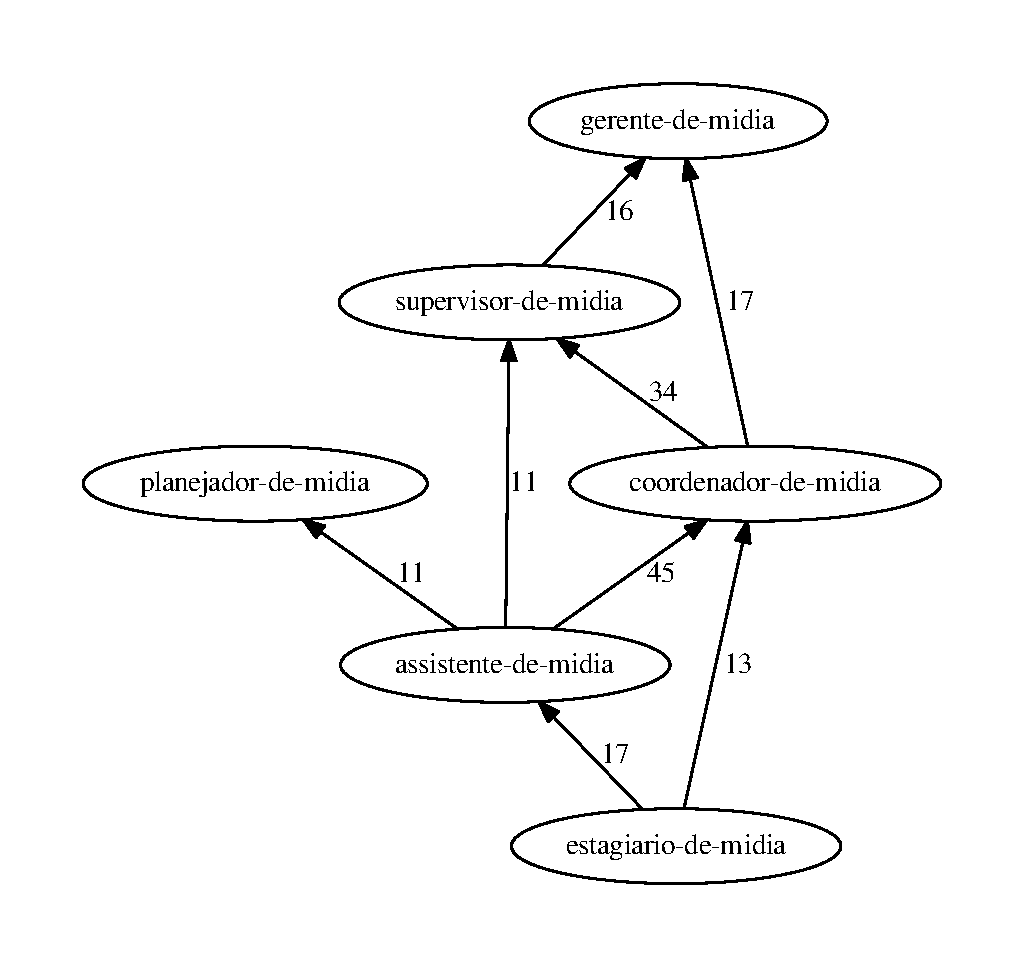
\includegraphics[scale=0.6]{cluster_23.pdf}
  \caption{Parte do MCar com ocupações relacionadas à carreira de mídia.}
  \label{fig:ex-mapa-midia}
\end{figure}

As ocupações no MCar foram definidas a partir de \textit{consenso} nos currículos. Como o título da ocupação é um campo em que o usuário digita livremente, assumiu-se que, se um grupo \enquote{suficientemente grande} de pessoas entra em acordo sobre uma certa nomenclatura, ela representa objetivamente uma ocupação. Essa abordagem é colocada de maneira implícita em ~\citeonline{Abbott1995-ft}, enquanto \citeonline{Gunz2007-hr} a exploram para definir fronteiras de carreiras.

Uma das maiores dificuldades para se estabelecer uma ocupação através de consenso está em definir o quanto ele deve ser \enquote{suficientemente grande} para que seja considerada como tal. Para os fins desse trabalho, esse número foi obtido de forma experimental e empírica. Para isso, procurou-se o número mínimo de repetições na grafia das ocupações de maneira que não fossem encontrados erros de digitação recorrentes, ou seja, que das ocupações criadas por consenso, nenhuma fosse mero resultado de erro. Esse número foi definido em 30 repetições da mesma grafia no título da ocupação.

Para a criação do MCar foram usados os currículos anonimizados de 10 milhões de usuários registrados no site VAGAS.com.br. A seleção de dados, bem como o processamento das informações, seguiu um procedimento conservador. Isso significa que as decisões tomadas em sua construção procuram minimizar os erros decorrentes da qualidade dos dados, mesmo que isso signifique trabalhar com uma quantidade menor deles. Utilizando o exemplo na Figura~\ref{fig:ex-mapa-midia}, isso significa que, provavelmente, muito mais do que 16 pessoas na base de dados fizeram a transição de \enquote{supervisor-de-midia} para a ocupação \enquote{gerente-de-midia}, porém, esses 16 são livres de erros e subjetividade.

Da massa de currículos, apenas os atualizados no período entre 2011 e 2016 foram usados. Currículos em duplicação foram removidos usando o CPF como identificador; em caso de duplicação, apenas o currículo mais recente foi considerado. Na impossibilidade de se verificar a duplicação, como por exemplo, na ausência do CPF, o currículo também foi descartado.

Finalmente, algumas informações gerais foram extraídas dos currículos que passaram pelo processo acima e o restante das informações foi descartada, incluindo quaisquer maneiras de se identificar a pessoa descrita no currículo, garantindo a anonimidade do processo.

As informações extraídas são o sexo, último salário, graduação (se existente) ou escolaridade, e a sequência de ocupações pela qual o profissional passou com seu título, descrição e período em que exerceu a ocupação. Esse trabalho utiliza apenas a sequência de ocupações.

O título da ocupação é um dos principais artefatos do MCar, é ele quem fornece a identidade para o nó. Como descrito acima, nos currículos, o título da ocupação é um campo de texto livre, ou seja, o usuário pode digitar o título sem restrições. Se por um lado isso permite a identificação de ocupações de nicho, novas ou que usem jargão de área, por outro significa que os títulos possuem erros de grafia, variações de gênero (como em \enquote{advogado} e \enquote{advogada} ou \enquote{moto boy} e \enquote{moto girl}), composição de múltiplas ocupações em um mesmo título (como \enquote{caixa/balconista}), abreviações e toda a gama de erros de interpretação possíveis.

As ocupações passam por um corretor ortográfico criado especificamente para esse trabalho, uma vez que um corretor tradicional não é capaz de identificar jargões de área como \enquote{enfermeiranda}, \enquote{rigger} ou \enquote{IRLA}.

Como exemplo, o dicionário do corretor possui cerca de 750 variações ortográficas que são traduzidas para o termo \enquote{auxiliar}, dentre eles, simples erros de omissão como \enquote{uxiliar}, até variações mais elaboradas como \enquote{ausciliar} e \enquote{alsilia}.

Após o trabalho de correção ortográfica, os títulos foram agrupados e contados. Especialistas da empresa verificaram os resultados dos maiores grupos para identificar anomalias, como ocupações com os títulos \enquote{sim}, \enquote{não} e \enquote{o mesmo}. Ocupações como essas foram excluídas do trabalho.

A partir desse ponto essa pesquisa diverge do MCar, usando os mesmos dados, mas processando-os de maneira diferente. Enquanto o segundo usa conexões direcionadas entre duas ocupações, o primeiro usa trigramas direcionados, ou seja, sequências de três ocupações.  Dessa forma, o algoritmo consegue identificar ocupações que pertencem a múltiplas comunidades. Os detalhes são explicados ainda nessa seção.

No MCar, a sequência de ocupação foi usada para gerar pares. Por exemplo, um currículo com a sequência de ocupações \enquote{saladeiro} $\to$ \enquote{chapeiro} $\to$ \enquote{cozinheiro} gera os pares \enquote{saladeiro} $\to$ \enquote{chapeiro} e \enquote{chapeiro} $\to$ \enquote{cozinheiro}. Os pares foram agrupados e sua contagem se torna o peso de cada conexão na rede final.

Finalmente, as conexões foram conectadas pela ocupações em comum e a rede final foi construída e armazenada em um banco de dados de grafo. Um sistema online\footnote{Disponível em \url{http://www.vagas.com.br/mapa-de-carreiras}} disponibiliza as informações publicamente. Apesar de gratuito e de consulta pública, os dados do Mapa VAGAS da Carreira não são de uso livre. A empresa gentilmente cedeu os dados ao pesquisador para esse trabalho.

Para essa pesquisa, são usado \textit{trigramas de ocupações} ao invés de conexões simples. Por exemplo, um histórico profissional com quatro ocupações como \enquote{saladeiro} $\to$ \enquote{chapeiro} $\to$ \enquote{cozinheiro} $\to$ \enquote{chef} gera dois trigramas \enquote{saladeiro} $\to$ \enquote{chapeiro} $\to$ \enquote{cozinheiro} e \enquote{chapeiro} $\to$ \enquote{cozinheiro} $\to$ \enquote{chef}. 

Históricos profissionais com apenas duas ocupações (bigramas) também são utilizadas. O trabalho usa preferencialmente trigramas, mas recorre a eles se não houver informação suficiente disponível. Históricos profissionais com apenas uma ocupação são descartados. Trigramas e bigramas com menos de 5 ocorrências são descartados.

Depois do processo de limpeza, a rede resultante foi analisada quanto ao número de componentes. Os resultados na Tabela~\ref{tab:componentes} indicam vários componentes com apenas um nó, alguns poucos com dois e três nós e um componente gigante. Os componentes menores foram descartados e apenas as ocupações presentes na ocupação gigante foram usados.

Os componentes com apenas um nó são sequências de ocupações que se repetem, por exemplo \enquote{engenheiro de tubulação} $\to$ \enquote{engenheiro de tubulação}, mas não possuem conexão com outras ocupações.

\begin{table}
    \centering
    \begin{tabular}{@{} c r @{}}
        \toprule
        Tamanho & Componentes \\
        \midrule
        1        &  1.087 \\
        2        &  19 \\
        3        &  1 \\
        7.267 &  1 \\
        \bottomrule
    \end{tabular}
    \caption{Tabela de frequência por tamanho de componente na rede.}
    \label{tab:componentes}
\end{table}

O rede final possui 7.267 ocupações e 145.115 conexões, sendo 68.771 bigramas e 76.344 trigramas.

Para caracterizar a rede na Seção~\ref{sec:resultados}, a rede foi convertida em uma rede sem memória, efetivamente unificando trigramas e bigramas em conexões direcionadas e ponderadas. A rede transformada possui as mesmas 7.267 ocupações com 73.064 conexões.

%===================================
\section{Grafos e Detecção de Comunidades} \label{sec:comunidades}
%===================================

Uma \textit{comunidade} é um subgrafo com conexões mais \textit{coesas} entre seus nós do que com nós do restante do grafo. A palavra \enquote{coesão} aqui pode ser interpretada de várias maneiras. Para \citeonline{Ahn2010-uh,Evans2009-lq}, uma comunidade é definida quando o número de conexões internas do subgrafo é maior que o número de conexões que o conecta ao resto do grafo. Para \citeonline{Barabasi2016-rn,Newman2004-jg} a comunidade deve possuir uma densidade de conexões mais alta do que o esperado em uma rede aleatória equivalente. Para esses autores, o número de conexões é o fator determinante para a identificação da comunidade.

\citeonline{Rosvall2009-sd} e \citeonline{Van_Dongen2000-qm}, por sua vez, trabalham a detecção de comunidades como a identificação de fluxos mais frequentes na rede. Assumindo que uma conexão representa um fluxo, comunidades possuem fluxo maior entre seus nós do que com outros fora da comunidade.

Essas abordagens distintas são aplicáveis a cenários diferentes. A densidade de conexões é mais adequada em redes onde a estrutura é importante, como, por exemplo, em uma rede social. Já em redes que representam fluxos, como circuitos ou redes de transporte, a segunda abordagem é mais atraente~\cite{Rosvall2009-sd}.

Para esse trabalho, a identificação de comunidades por fluxo é adequada por concepção. Como exposto na Seção~\ref{sec:carreira}, as fronteiras de carreira são definidas pelo consenso das movimentações profissionais: transições menos frequentes definem essas fronteiras.

Essa frequência é relativa ao fluxo entre os nós próximos: dez transições para uma ocupação como \enquote{Auxiliar Administrativo}, que possui dezenas de milhares de profissionais entrando e saindo, não tem a mesma importância que para \enquote{Assistente de Mídia} (Figura~\ref{fig:ex-mapa-midia}), em que essa dezena representa mais de 10\% das transições registradas.

O algoritmo Infomap (detalhado na Seção~\ref{sec:infomap}) utiliza \textit{random walkers} para identificar comunidades. Os caminhos em que eles circulam mais frequentemente são considerados como fazendo parte da mesma comunidade; por outro lado, caminhos raramente utilizados definem as fronteiras entre uma comunidade e outra, de maneira análoga à concepção de fronteiras de carreira de~\citeonline{Gunz2007-hr}.

Portanto, por analogia, a identificação de comunidades do algoritmo Infomap identifica fronteiras de carreiras em uma rede em que as conexões representam o fluxo de profissionais entre ocupações, como é o caso do MCar.

Nesse trabalho, as comunidades são chamadas \textit{ilhas ocupacionais}.

%===================================
\subsection{O Algoritmo Infomap} \label{sec:infomap}
%===================================

Segundo \citeonline{Grunwald2007-bt}, quaisquer regularidades em um conjunto de dados podem ser usadas para comprimi-los, ou seja, descrevê-los usando uma quantidade menor de símbolos. Quanto maior a regularidade, maior a compressão, dessa forma, dentre várias representações possíveis dos dados, a que apresentar maior compressão é também aquela que melhor identifica padrões nos dados. A Descrição de Comprimento Mínimo (\textit{Minimum Description Length}) é a disciplina que estuda essa relação~\cite{Grunwald2007-bt}.

O algoritmo Infomap aproveita essa dualidade entre detecção de padrões e compressão de dados para identificar padrões de fluxo em redes~\cite{Rosvall2009-sd}.

Para compreender o algoritmo, é preciso entender como um trajeto aleatório em uma rede é representado e como a Descrição de Comprimento Mínimo usa essa representação na detecção de comunidades.

Para isso, descreve-se o caminho que um \textit{random walker} faz em uma rede através da sequência de nós pela qual ele passa. Por exemplo, assumindo uma rede com os nós $A$, $B$ e $C$, um caminho possível poderia ser descrito por $ABACBA$.

A Figura~\ref{fig:graph01} mostra um grafo regular, onde todos os nós possuem três vizinhos. Nesse tipo de rede, um \textit{random walker} ergódico (de caminho infinito) percorre todas as conexões o mesmo número de vezes. A Figura~\ref{fig:walk01} mostra um caminho aleatório passando por 800 nós.

\begin{figure}[ht]
  \centering
  \subfloat[][Rede regular] {
    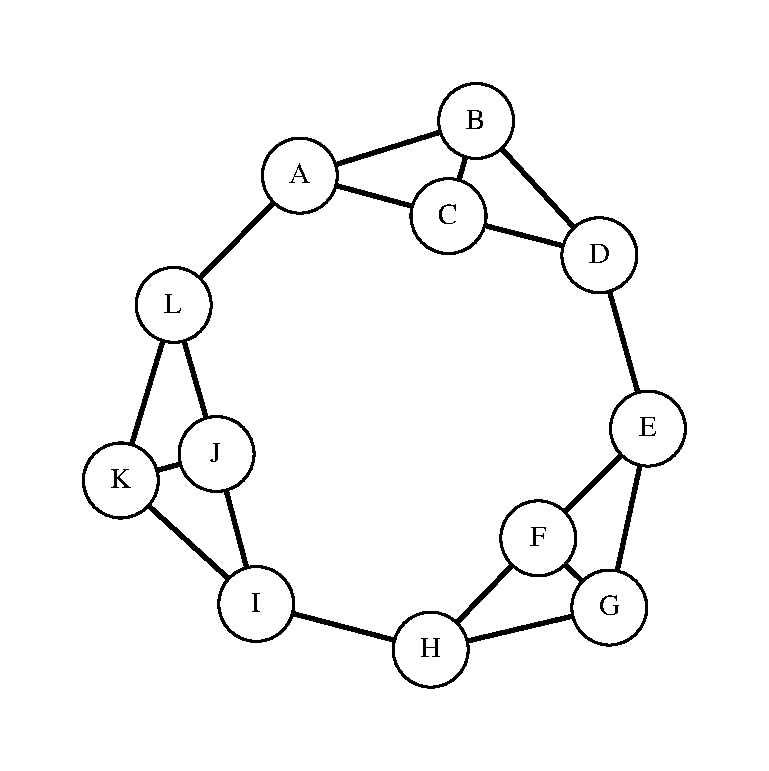
\includegraphics[scale=0.4]{graph01.pdf}
    \label{fig:graph01}
  }
  \subfloat[][Caminho na rede] {
    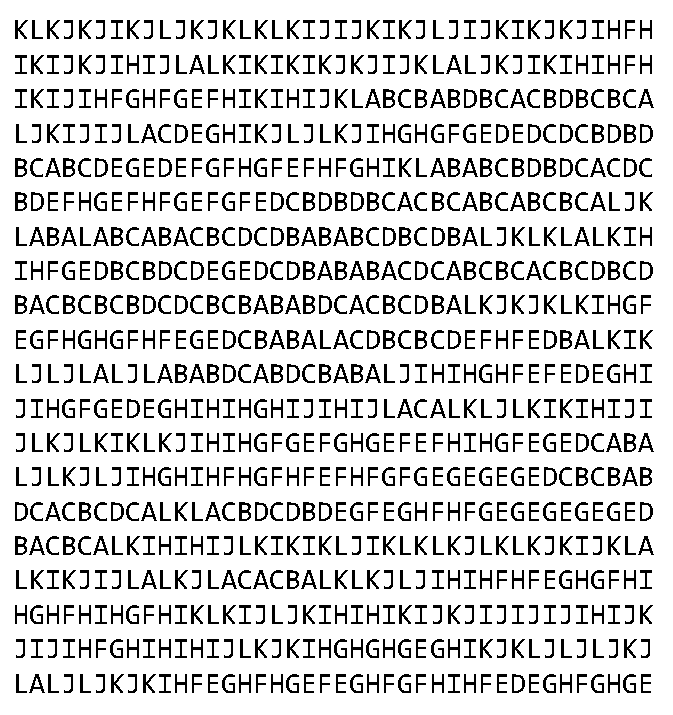
\includegraphics[scale=0.4]{graph01_path.pdf}
    \label{fig:walk01}
  }    
  \caption{Caminho de um \textit{random walker}}
\end{figure}

Apesar de ser uma rede regular, onde cada nó possui três conexões, sua topologia faz com que o \textit{random walker} fique \enquote{preso} nos grupos formados pelos nós $ABCD$, $EFGH$ e $IJKL$; escapando esporadicamente de um para outro, onde circula até escapar novamente. Esses grupos são destacados na Figura~\ref{fig:graph02}. O caminho percorrido pelo \textit{walker} é exibido na Figura~\ref{fig:walk02}, dessa vez destacando os grupos por onde ele passa. As cores em ambas as figuras torna fácil perceber seu comportamento.

\begin{figure}[ht]
  \centering
  \subfloat[][Rede regular] {
    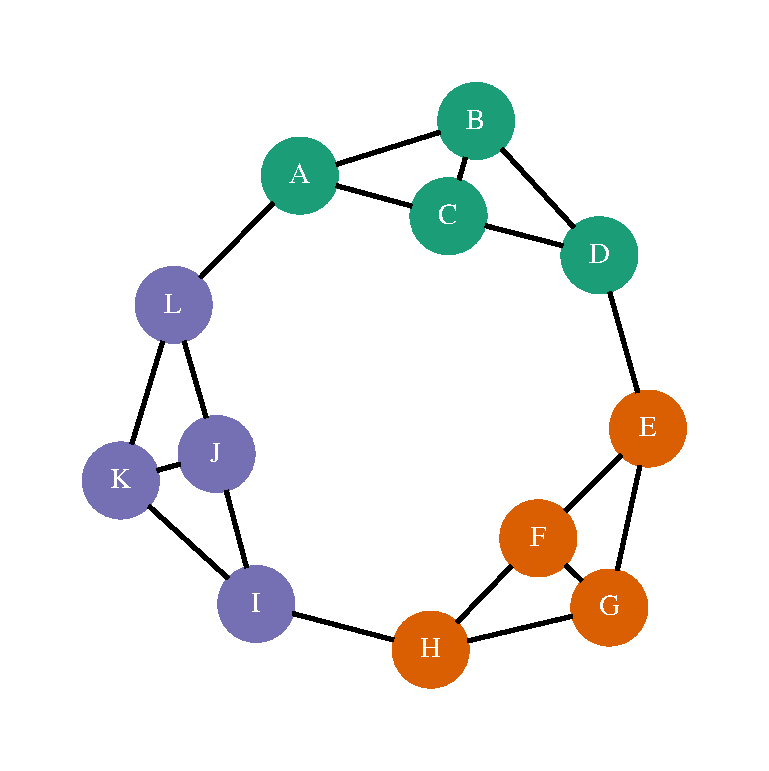
\includegraphics[width=0.4\linewidth]{graph02.pdf}
    \label{fig:graph02}
  }
  \subfloat[][Caminho na rede] {
    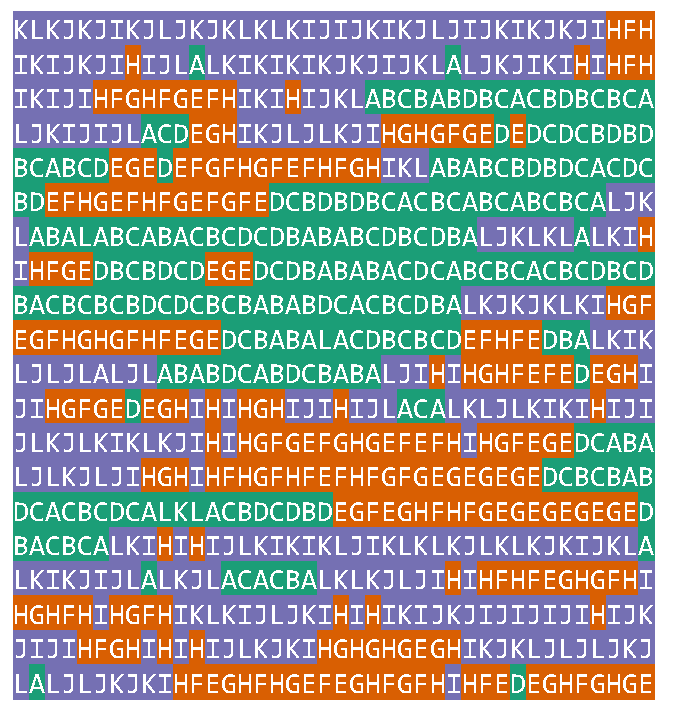
\includegraphics[width=0.4\linewidth]{graph02_path.pdf}
    \label{fig:walk02}
  }    
  \caption{Rede e caminho destacados}
\end{figure}

Se cada nó for representado por uma sequência de bits, podemos medir quanta informação é necessária para representar o caminho feito pelo \textit{random walker}. Usando a codificação de tamanho variável de  \citeonline{Huffman1952-ak} os nós mais frequentes são representados por códigos menores, resultando em uma codificação menor para representar um caminho do que uma que use códigos de tamanho fixo.

Os códigos usados por cada grupo são chamados \textit{codebooks}, os códigos que indicam qual \textit{codebook} será usado também é um \textit{codebook}, funcionando como um índice. Na Figura~\ref{fig:graph04}, existem três deles, um para cada grupo, contendo os nós \enquote{00}, \enquote{01}, \enquote{10}, \enquote{110} e o código de saída \enquote{111}. O \textit{codebook} índice possui os códigos: \enquote{0}, \enquote{10} e \enquote{11}.

Dessa forma, sem o uso de \textit{codebooks}, o caminho que começa no nó mais abaixo do grafo da Figura~\ref{fig:graph03} e termina no nó do canto superior esquerdo é descrito pela sequência binária \enquote{000 1110 1011 1111 1101}, usando 19 bits. O mesmo caminho, usando a codificação com \textit{codebooks} da Figura~\ref{fig:graph04} é \enquote{\textbf{0} 01 110 \textit{111} \textbf{11} 00 01 10} e possui 17 bits (os números em negrito indicam entrada em um grupo e o número em itálico indica saída do grupo).

Nesse caminho curto, ambas as codificações têm tamanhos similares, Porém, em um caminho infinitamente longo (ergódico), o uso de múltiplos \textit{codebooks} pode produzir um código mais compacto do que o uso de um único \textit{codebook}. Como exemplo, o caminho da Figura~\ref{fig:walk01} usando a codificação com um único \textit{codebook} da Figura~\ref{fig:graph03} possui 2880 bits contra 1776 bits usando a codificação com três \textit{codebooks} da Figura~\ref{fig:graph04}.

\begin{figure}[ht]
  \centering
  \subfloat[][Nós usando codificação de Huffman] {
    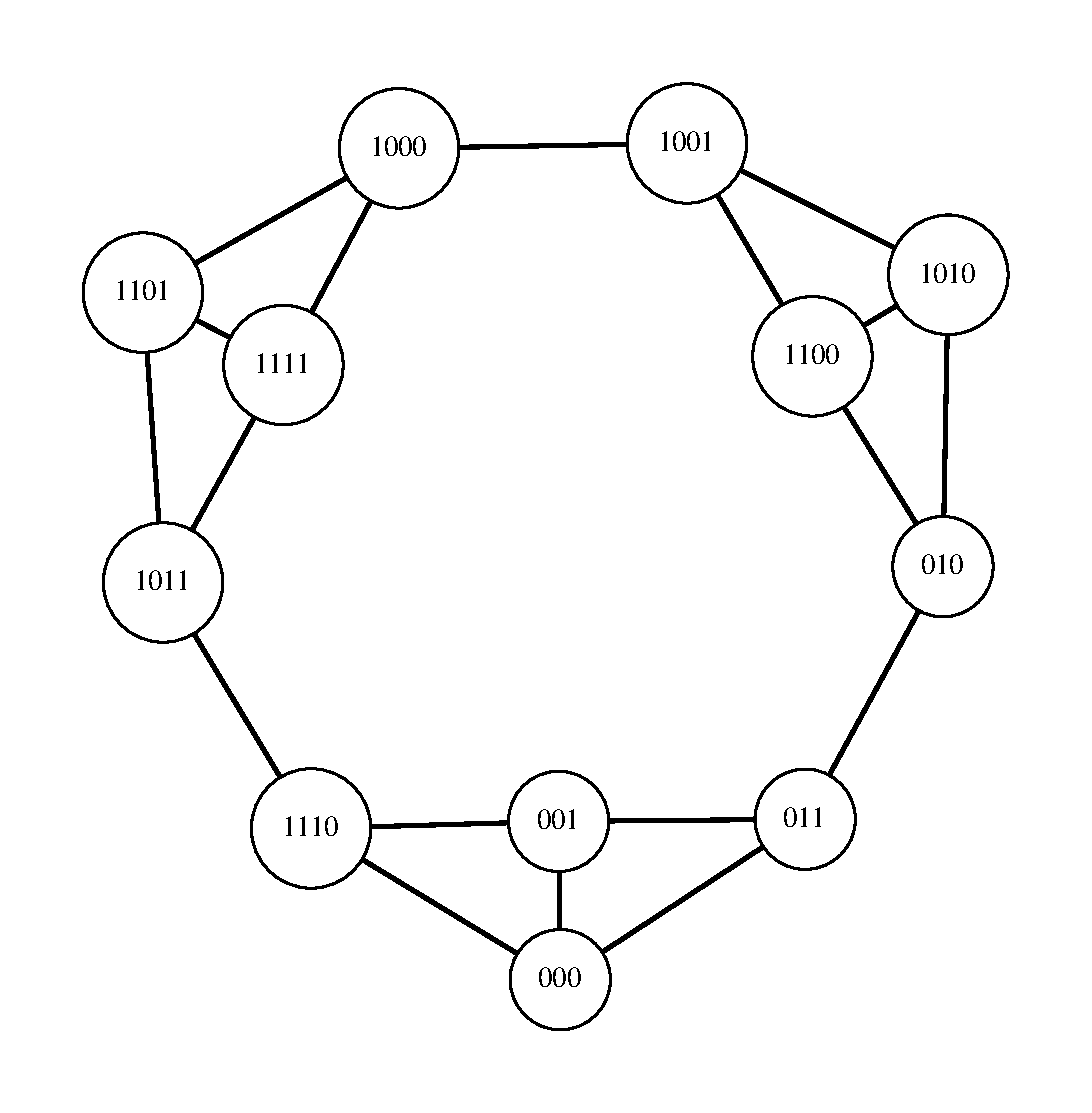
\includegraphics[width=0.4\linewidth]{graph03.pdf}
    \label{fig:graph03}
  }
  \subfloat[][Reaproveitamento de códigos] {
    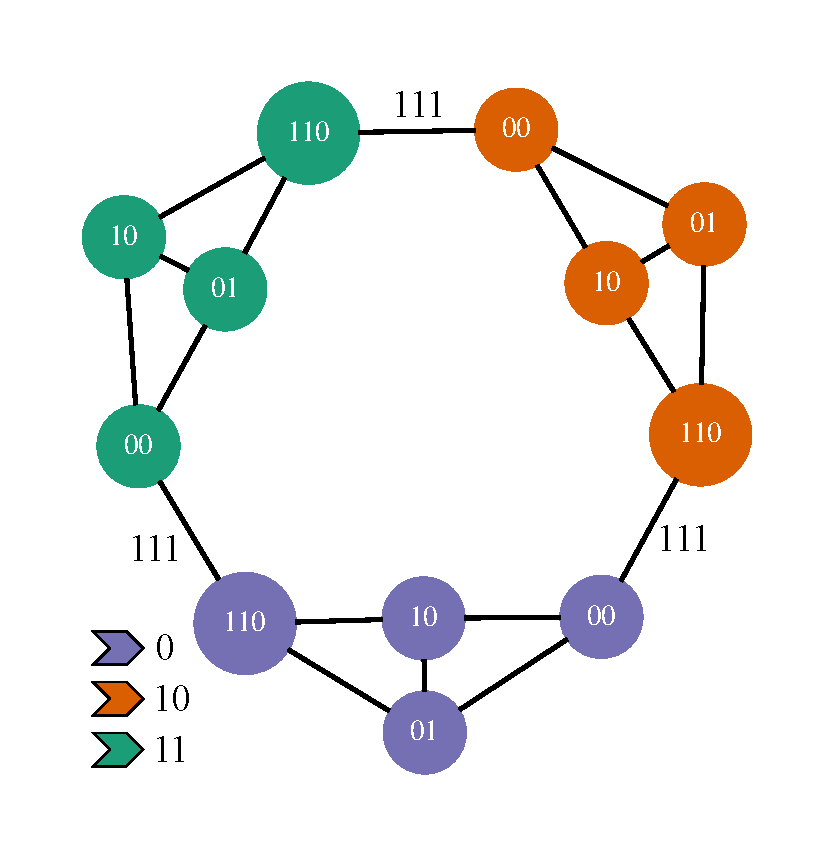
\includegraphics[width=0.4\linewidth]{graph04.pdf}
    \label{fig:graph04}
  }    
  \caption{Codificação dos nós}
\end{figure}

O particionamento da rede em grupos onde os caminhos aleatórios podem ser representados da maneira mais compacta possível deve representar o melhor particionamento em relação ao fluxo.

A \enquote{Equação de Mapa}\footnote{No original: \textit{Map Equation}}~\cite{Rosvall2009-sd} permite que se identifiquem as menores codificações possíveis para um determinado particionamento da rede sem a necessidade de se empregar \textit{random walkers} de fato. Com ela, a detecção de comunidades usando o fluxo como critério de coesão se reduz a um problema de otimização.

A Equação de Mapa é
\begin{equation} \label{eq:map-equation}
  L(\mathsf{M}) = q_\curvearrowright H(\mathcal{Q}) + \sum_{i \in \mathsf{M}} p^i_\circlearrowright H(\mathcal{P}^i)\,,
\end{equation}
onde $L(\cdot)$ é o menor tamanho de codificação possível para representar um certo particionamento; $\mathsf{M}$ é o particionamento dos nós em comunidades $i \in \mathsf{M}$; $q_\curvearrowright$ é a probabilidade de um \textit{random walker} sair de qualquer comunidade e passar para o \textit{codebook} índice; $H(\mathcal{Q})$ (\textit{eta} em maiúsculo) é número médio de bits usado para representar o \textit{codebook} índice segundo a distribuição de probabilidade $\mathcal{Q}$; e $H(\mathcal{P}^i)$ também é o número médio de bits, mas dessa vez daqueles usados na comunidade $i$ segundo a distribuição $\mathcal{P}^i$; finalmente $p^i_\circlearrowright$ é a probabilidade do \textit{walker} estar na comunidade $i$.

$H(\textbf{p})$ é a equação que descreve a entropia da informação segundo uma certa distribuição de probabilidade $\textbf{p}$~\cite{Shannon1948-ic}. Ela se refere a média de bits necessária, por símbolo, para se representar a informação gerada por um processo estocástico e é expressa como:
\begin{equation*}
H(\textbf{p}) = - \sum_\alpha p_\alpha \log_2 p_\alpha\,.
\end{equation*}

Nessa equação, $p_\alpha$ é a probabilidade estacionária da rede, ou seja, em um caminho infinito, qual fração de tempo o \textit{walker} estaria em $\alpha$~\cite{Rosvall2009-sd}.

Para calcular $p_\alpha$ inicia-se com a matriz estocástica linear $W$, gerada a partir da matriz de adjacência $A$ direcionada e ponderada. Em uma matriz estocástica linear, a soma dos pesos de entrada do nó (linha) é normalizado para que resulte em 1. Cada elemento $w_{\alpha \beta}$ dessa matriz representa a probabilidade de um \textit{random walker}  em $\alpha$ chegar ao nó $\beta$.  Transportada para a realidade do MCar, essa é a probabilidade de alguém na ocupação $\alpha$ fazer a transição para a ocupação $\beta$.

Sendo $n$ o número de nós da rede, define-se $w_{\alpha \beta}$ como:
\begin{align} \label{eq:matriz-estocastica}
w_{\alpha \beta} = 
    \begin{cases*}
        \frac{1}{n}, & \text{se $\alpha$ não possui conexões de saída, ou seja, $\sum_\beta A_{\alpha \beta} = 0$,} \\
        0, & \text{se não há conexão entre $\alpha$ e $\beta$,} \\
        \frac{A_{\alpha \beta}}{\sum_\beta A_{\alpha \beta}}, & \text{caso contrário.}
    \end{cases*}
\end{align}

A primeira cláusula da Equação~\ref{eq:matriz-estocastica} garante que a matriz estocástica possua linhas totalizando 1 quando o nó não possui conexões de saída. Para efeitos do \textit{random walker}, isso significa que ele se teleporta para um nó qualquer da rede quando se encontra em um nó sem saída. Caso contrário, os nós sem conexões de saída acumulariam a probabilidade total da rede~\cite{Page1999-ag}.

A probabilidade estacionária $p_\alpha$ é calculada pelo sistema de equações
\begin{equation} \label{eq:page-rank}
p_\alpha = \frac{1}{n} \tau + \sum_\beta (1 - \tau) p_\beta w_{\beta \alpha}\,,
\end{equation}
onde $\tau$ é a probabilidade do \textit{walker} ser teleportado para um nó aleatório. A primeira cláusula da Equação~\ref{eq:matriz-estocastica} e a presença de $\tau$ transformam o \textit{random walker} em um \textit{random surfer}. Esse artifício foi usado por~\citeonline{Page1999-ag} na criação do algoritmo de PageRank e fornece a base para a Equação de Mapa.

O recurso de teleporte garante a ergodicidade do caminho e, segundo o teorema de Perron-Frobenius, faz com que a probabilidade estacionária seja definida~\cite{Rosvall2009-sd}.

A partir de $p_\alpha$, é possível expandir a Equação de Mapa.

Sendo $q_{i \curvearrowright}$ a probabilidade de saída da comunidade $i$ e $q_{\curvearrowright}$ a probabilidade de saída de qualquer comunidade, o valor de $q_{\curvearrowright}$ equivale à taxa de uso do \textit{codebook} índice, uma vez que a saída de uma comunidade implica  em seu uso para indicar qual a próxima comunidade.

Finalmente, sendo $n$ o número de nós da rede e $n_i$ o número de nós pertencente à comunidade $i$, expande-se a Equação~\ref{eq:map-equation} em
\begin{align}
q_{i \curvearrowright} &= \frac{n - n_i}{n} \tau \sum_{\alpha \in i} p_\alpha + (1 - \tau) \sum_{\alpha \in i} \sum_{\beta \nin i} p_\alpha w_{\alpha \beta} \nonumber \\
q_\curvearrowright       &= \sum_{i \in M} q_{i\curvearrowright} \nonumber \\
p^i_\circlearrowright    &= q_{i \curvearrowright} + \sum_{\alpha \in i} p_\alpha \nonumber \\
H(\mathcal{Q})            &= - \sum_{i \in M} \frac{q_{i \curvearrowright}}{q_\curvearrowright} \log_2 \frac{q_{i \curvearrowright}}{q_\curvearrowright} \nonumber \\
H(\mathcal{P}^i)         &= - \frac{q_{i \curvearrowright}}{p^i_\circlearrowright} \log_2 \frac{q_{i \curvearrowright}}{p^i_\circlearrowright} 
-  \sum_{\alpha \in i} \frac{p_\alpha}{p^i_\circlearrowright} \log_2  \frac{p_\alpha}{p^i_\circlearrowright} \label{eq:eta-p} \\
L(\mathsf{M})              &= q_\curvearrowright \log_2 q_\curvearrowright - 2 \sum_{i = 1}^m q_{i \curvearrowright} \log_2 q_{i \curvearrowright} - \sum_{\alpha = 1}^n p_\alpha \log_2 p_\alpha + \sum_{i = 1}^m p^i_\circlearrowright \log_2 p^i_\circlearrowright\,. \nonumber
\end{align}

\subsection{Redes com Memória}  \label{sec:redes-com-memoria}

Na modelagem do MCar, um \enquote{Analista de Sistemas} e um \enquote{Arquiteto} têm chances similares de se tornarem \enquote{Coordenador de Projetos}. Entretanto, apesar de receber o mesmo nome, as competências de um coordenador de projetos da área de software e de arquitetura são bastante diferentes. Na realidade, essa é uma ocupação que pode figurar em duas ilhas ocupacionais bastante distintas pois a movimentação entre essas duas áreas é relativamente rara em comparação com a movimentação dentro de si mesmas.

O padrão esperado nesse caso, é que profissionais de cada ilha vão para essa \enquote{Gerente de Projetos} e voltem para outras de sua própria ilha ao invés de cruzar a fronteira de carreira. Para poder identificar esse padrão, é preciso considerar não apenas o trabalho imediatamente anterior, mas também o subsequente.

No MCar as ocupações prévias do profissional não influenciam seu próximo passo, apenas sua ocupação atual. No entanto, como exemplificado no caso acima, a \enquote{perda de memória} da ocupação anterior compromete a identificação das comunidades.

Efetivamente, o MCar modela o fluxo de profissionais como um cadeia de Markov de primeira ordem. Considerar ocupações anteriores transforma o fluxo da rede em uma cadeia de Markov de ordem superior ou \enquote{Redes com Memória}\footnote{no original: \textit{Memory Networks}} \cite{Edler2017-kt}.

\begin{figure}[htb]
    \centering
    \subfloat[][Simples] {
        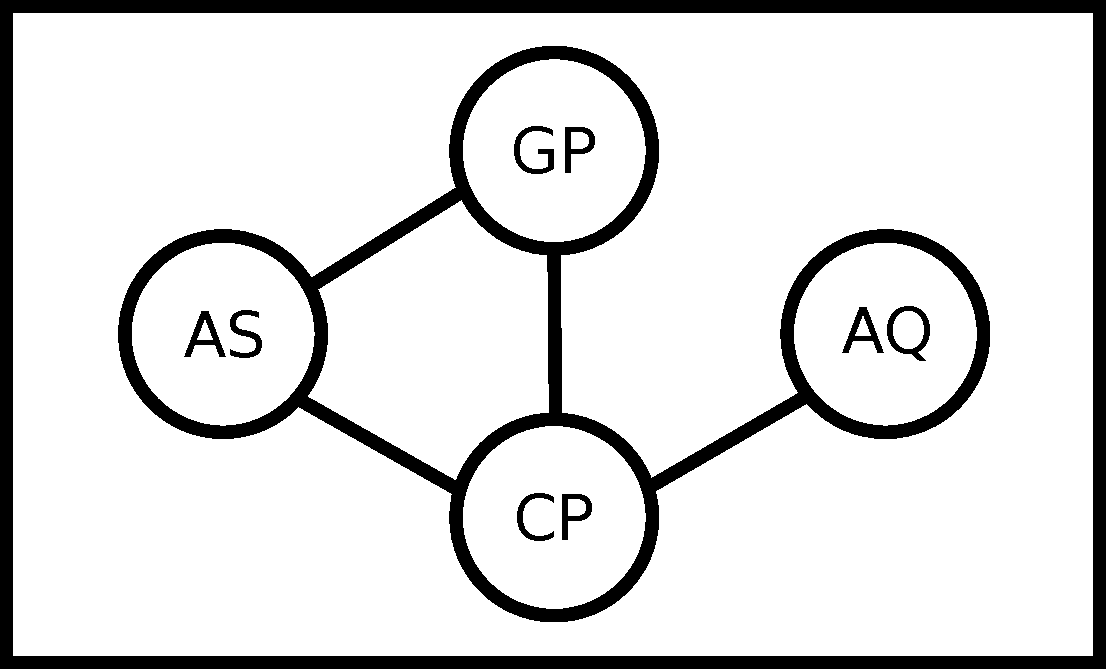
\includegraphics[width=0.3\linewidth]{ex-multilayer-04.pdf}
        \label{fig:ex-multilayer-simples}
    }
    \subfloat[][Direcionada]{
        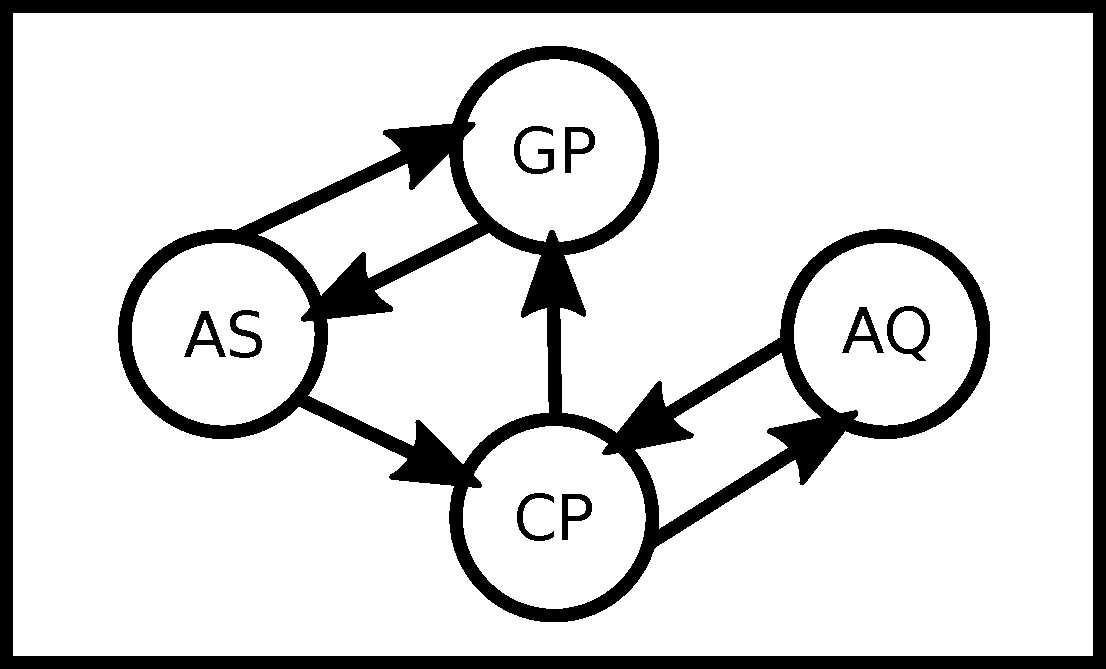
\includegraphics[width=0.3\linewidth]{ex-multilayer-05.pdf}
        \label{fig:ex-multilayer-direcionada}
    }
    \subfloat[][Trigramas] {
        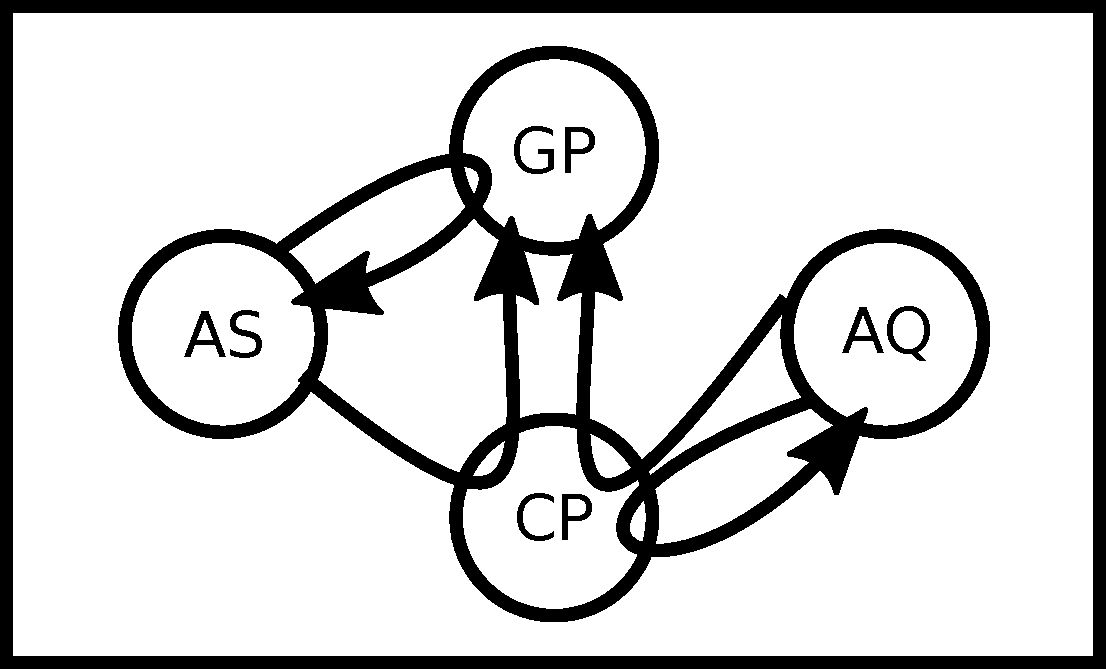
\includegraphics[width=0.3\linewidth]{ex-multilayer-01.pdf}
        \label{fig:ex-multilayer-trigrama}
    }
    \caption{Exemplo de uma rede com 4 nós e representações com sucessivos aumentos de informação. Os nós são GP - \textit{Gerente de Projetos}, AS - \textit{Analista de Sistemas}, AQ - \textit{Arquiteto} e CP - \textit{Coordenador de Projetos}. A rede simples da Figura~\ref{fig:ex-multilayer-simples} faz as conexões entre AS e CP agirem como bidirecionais; a rede direcionada da Figura~\ref{fig:ex-multilayer-direcionada} unifica as probabilidades de um \textit{random-walker} caminhar entre CP e GP, ignorando onde estava anteriormente. Os fluxos com dois níveis de memória (processo markoviano de segunda ordem) podem ser observados na Figura~\ref{fig:ex-multilayer-trigrama}}
\end{figure}

\citeonline{Edler2017-kt} adaptam a Equação de Mapa  para trabalhar com  Redes com Memória transformando-as em uma rede multi-camadas em uma representação chamada \enquote{Rede com Memória em Multi-Camadas}\footnote{no original: \textit{Multilayer Memory Network}}. Um rede multi-camadas é usada para representar redes em sistemas complexos onde existem contextos diferentes de relacionamento~\cite{Kivela2014-pb}. Por exemplo, em uma rede social onde pessoas participam de vários eventos, cada camada pode representar um evento, enquanto os relacionamentos podem representar a interação entre elas em cada evento. 

\begin{figure}[htb]
    \centering
    \subfloat[][Trigramas] {
        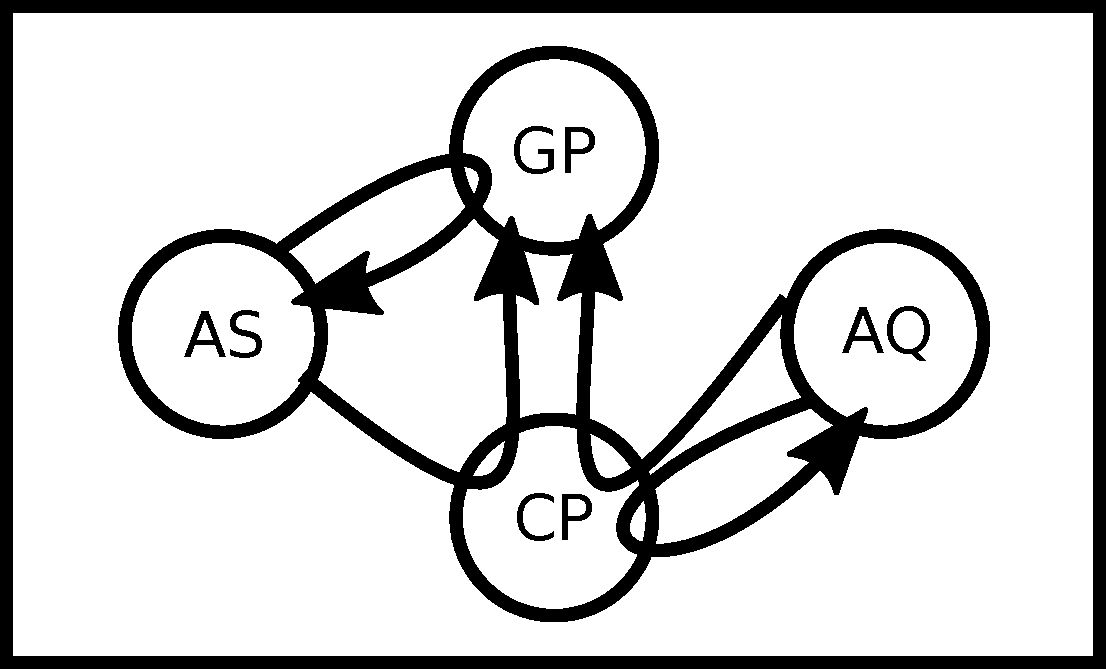
\includegraphics[width=0.3\linewidth]{ex-multilayer-01.pdf}
        \label{fig:ex-multilayer1}
    }
    \subfloat[][Como camadas] {
        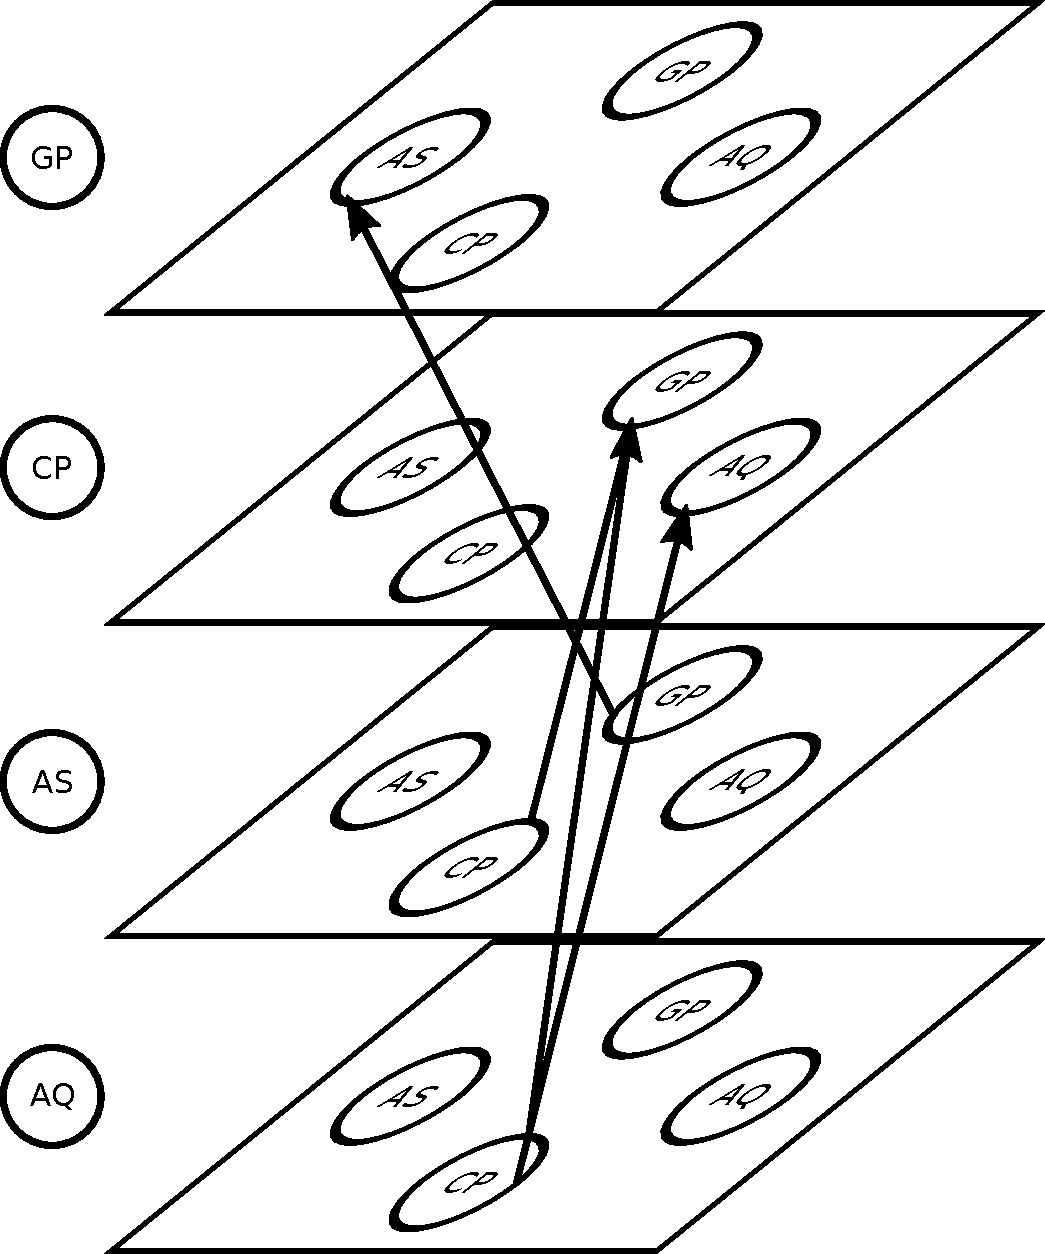
\includegraphics[width=0.3\linewidth]{ex-multilayer-02.pdf}
        \label{fig:ex-multilayer2}
    }
    \subfloat[][Projeção] {
        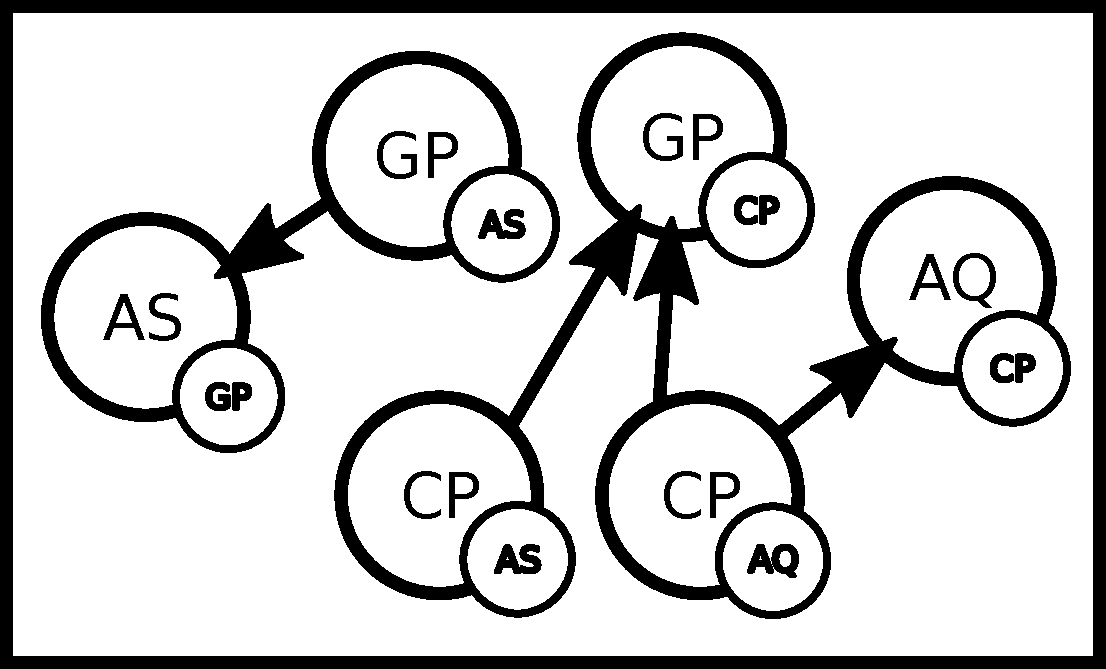
\includegraphics[width=0.3\linewidth]{ex-multilayer-03.pdf}
        \label{fig:ex-multilayer3}
    }
    \caption{Exemplo de uma rede com 4 nós e 4 trigramas (8 conexões). Os nós são GP - \textit{Gerente de Projetos}, AS - \textit{Analista de Sistemas}, AQ - \textit{Arquiteto} e CP - \textit{Coordenador de Projetos}. A mesma rede usando camadas para representar dois níveis de memória é exibida na Figura~\ref{fig:ex-multilayer2}, cada camada representa o nó anterior da conexão e cada imagem do nó na camada é chamado de \textit{nó-estado}. A projeção das camadas de volta para uma rede de camada única está na Figura~\ref{fig:ex-multilayer3}, as anotações em cada nó indicam a camada daquele nó-estado.}
    \label{fig:ex-multilayer-camadas}
\end{figure}

O exemplo da Figura~\ref{fig:ex-multilayer-camadas} mostra a rede formada pelas ocupações \enquote{Arquiteto}, \enquote{Analista de Sistemas}, \enquote{Coordenador de Projetos} e \enquote{Gerente de Projetos} e suas representações em camadas. A partir dessa representação é possível projetar uma rede de uma única camada (uma rede \enquote{comum}), criando-se um \textit{nó-estado} para cada nó em cada camada. Ignorando-se nós-estado que não possuem conexões, essa projeção cria um nó-estado para cada conexão de entrada, como pode ser observado na Figura~\ref{fig:ex-multilayer3}.

Um vez que a probabilidade estacionária é calculada através das conexões de saída, os nós-estado que possuem saída para os mesmos nós podem ser unificados sem perda de informação para identificação de comunidades. No exemplo da Figura~\ref{fig:ex-multilayer3}, a os nós $\text{CP}_\text{AS}$ e $\text{CP}_\text{AQ}$ podem ser unidos em um único nó. \citeonline{Edler2017-kt} chamam esse simplificação de Rede com Memória Esparsa\footnote{no original: \textit{Sparse Memory Network}}.

\begin{figure}[htb]
    \centering
    \subfloat[][Projeção] {
        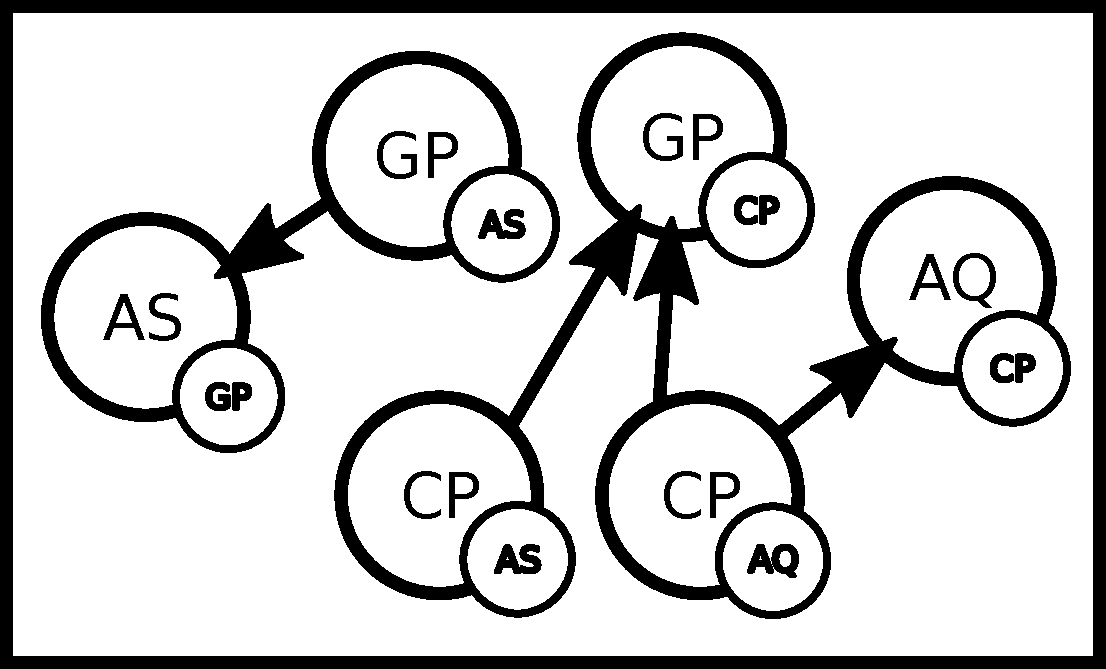
\includegraphics[width=0.3\linewidth]{ex-multilayer-03.pdf}
        \label{fig:ex-multilayer-projecao}
    }
    \subfloat[][Rede com Memória Esparsa] {
    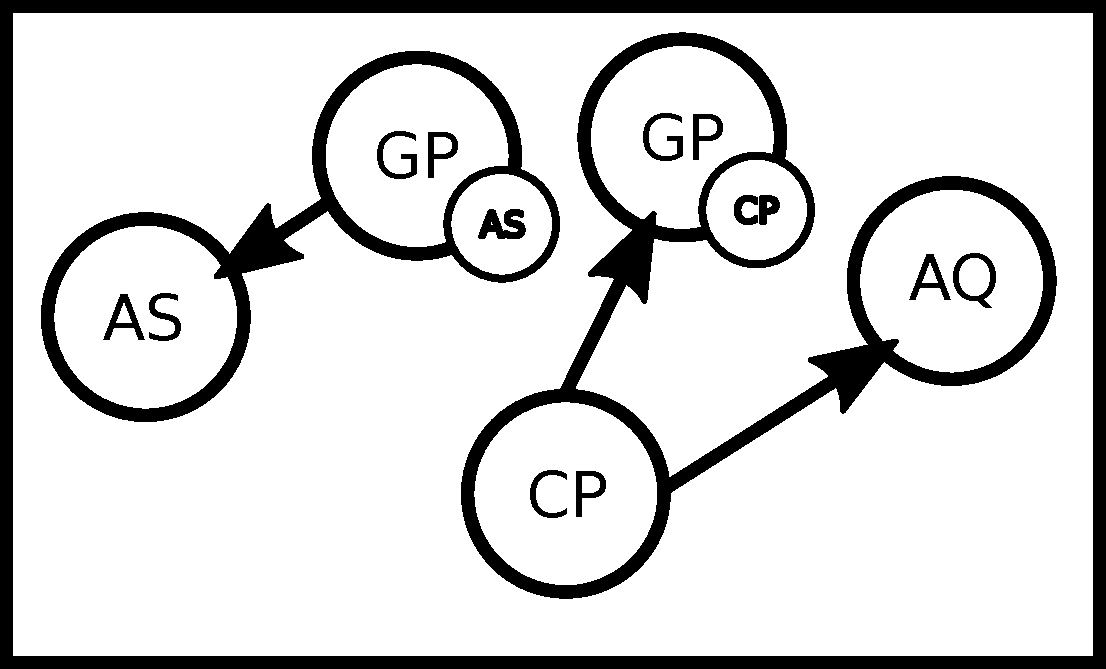
\includegraphics[width=0.3\linewidth]{ex-multilayer-06.pdf}
    \label{fig:ex-multilayer-esparsa}
}
    \caption{A rede pode ser simplificada unificando nós que possuem saída para os mesmos nós-estados, criando uma Rede com Memória Esparsa~\cite{Edler2017-kt}}
    \label{fig:ex-multilayer-memoria}
\end{figure}

Dessa forma, a aplicação da Equação de Mapa (Equação \ref{eq:map-equation}) permanece a mesma, bastando que os nós-estado que permanecem na mesma comunidade compartilhem o mesmo código. Para isso, a probabilidade estacionária $p_{\alpha_i}$ do nó $\alpha$ na comunidade $i$ passa ser a soma das probabilidades dos nós-estado $\alpha^s$ de $\alpha$ que estão na mesma comunidade $i$ em qualquer camada $S$,

\begin{equation*} \label{eq:page-rank-multilayer}
\pi_{\alpha_i} = \sum_{s \in S} p_{\alpha_i^s}\,.
\end{equation*}

Substituindo a probabilidade estacionária na Equação~\ref{eq:eta-p}, $H(\mathcal{P}^i)$ passa a ser

\begin{equation*}
H(\mathcal{P}^i) = - \frac{q_{i \curvearrowright}}{p^i_\circlearrowright} \log_2 \frac{q_{i \curvearrowright}}{p^i_\circlearrowright} 
-  \sum_{\alpha \in i} \frac{\pi_{\alpha_i}}{p^i_\circlearrowright} \log_2  \frac{\pi_{\alpha_i}}{p^i_\circlearrowright}\,.
\end{equation*}

\begin{comment}
% NOTA Ronie: E esse pedaço caiu também pq usei a equação do artigo mais recente do Rosvall. A frustração é que demorei duas (ou três) semanas pra entender e combinar as equações de 3 artigos em uma coisa que fizesse sentido >_<''  Ai... ai... 

====
\subsubsection{Variação com Sobreposição de Comunidades}

Para o algoritmo que permite que os nós pertençam a mais de uma comunidade, \citeonline{Viamontes_Esquivel2011-it} usam \textit{conexões com memória} para lembrar o passo anterior do \textit{random walker}. Quando ele se mover para um nó que pertence à múltiplas comunidades, ele se manterá na comunidade de onde veio, se possível.

Para isso, duas alterações são feitas na Equação de Mapa: mudança da definição de $p_\alpha$ para considerar nós em múltiplas comunidades (detalhada na Equação~\ref{eq:page-rank-overlap}) e a soma das probabilidades condicionais desses nós (detalhada na Equação~\ref{eq:map-equation-overlap}).

Na equação original, a probabilidade estacionária $p_\alpha$ de um \textit{random walker} estar em um nó $\alpha$ é dada pelo Equação~\ref{eq:page-rank}. Na variação com sobreposição, cada nó $\alpha$ possui uma probabilidade separada de estar em uma comunidade $i$, a probabilidade estacionária $p_{\alpha_i}$ é resolvida pelo sistema de equações
\begin{equation} \label{eq:page-rank-overlap}
p_{\alpha_i} = \sum_\beta \sum_{j \in M_\beta} p_{\beta_j} \delta_{\alpha_i \beta_j} \left[ (1 - \tau)  w_{\beta \alpha} + \frac{1}{n} \tau \right],
\end{equation}
onde $\delta_{\alpha_i \beta_j}$ é a função de transição entre comunidades, definida como
\begin{equation*}
\delta_{\alpha_i \beta_j} =
    \begin{cases*}
    1,                              & \text{se $i = j$},\\
    \frac{1}{|M_\beta|} & \text{se $i \neq j$ e $i \notin M_\beta$},\\
    0,                              & \text{se $i \neq j$ e $i \in M_\beta$}.
    \end{cases*}
\end{equation*}

A Equação de Mapa para comunidades com sobreposição é
\begin{equation} \label{eq:map-equation-overlap}
    L(\mathsf{M}) = q_\curvearrowleft \log_2 q_\curvearrowleft
                               - 2 \sum_{i=1}^m q_{i \curvearrowright} \log_2 q_{i \curvearrowright}
                               - \sum_{i=1}^m \sum_{\alpha \in i} p_{\alpha_i} \log_2  p_{\alpha_i}
                               + \sum_{i=1}^m p^i_\circlearrowright \log_2 p^i_\circlearrowright\,.                            
\end{equation}
\end{comment}

\begin{comment}
%% NOTA (Ronie): Tive problemas com o software para rodar a versão hierárquica SEM sobreposição. Para evitar alongar ainda mais esse artigo, excluí as partes de hierarquia. Não vai fazer muita falta, até pq o foco aqui são as ilhas (e não 'ilhas aninhadas').

Deixei o texto aqui embaixo por via das dúvidas.
====

A variação hierárquica do algoritmo possibilita detecção de comunidades aninhadas, nesse caso, ela é uma generalização da Equação de Mapa original que permite múltiplos \textit{codebooks} índices.

Nessa variação, cada partição $\mathsf{M}$ possui um subparticionamento $\mathsf{M}^i$. Cada um dos subgrupos de $\mathsf{M}^i$ possui outro subparticionamento $\mathsf{M}^{ij}$ e assim sucessivamente até o particionamento final $\mathsf{M}^{ij \ldots k}$.

A Equação de Mapa hierárquica é
\begin{equation} \label{eq:map-equation-hierarchical}
      L(\mathsf{M}) = q_\curvearrowright H(\mathcal{Q}) + \sum_{i \in \mathsf{M}} L(\mathsf{M}^i),
\end{equation}
com os níveis intermediários
\begin{equation*}
    L(\mathsf{M}^i) = q_\curvearrowright^i H(\mathcal{Q}^i) + \sum_{j \in \mathsf{M}^i} L(\mathsf{M}^{ij}),
\end{equation*}
e com os níveis finais
\begin{equation*}
    L(\mathsf{M}^{ij \ldots k}) = p_\circlearrowright^{ij \ldots k} H(\mathcal{P}^{ij \ldots k}).
\end{equation*}

A Equação de Mapa original (Equação~\ref{eq:map-equation}) é na verdade um caso específico da Equação~\ref{eq:map-equation-hierarchical}. Também é possível notar que a Equação de Mapa com sobreposição (Equação~\ref{eq:map-equation-overlap}) pode ser aplicada junto à variação hierárquica, resultando em uma versão hierárquica que permite que os nós pertençam a mais de um grupo.


%% SE USAMOS AS VARIAÇÕES DA EQUAÇÃO DE MAPA, ENTÃO PRECISAMOS APRESENTÁ-LAS AQUI
% Ronie: Feito!!!! Demorou uma vida pra entender como as equações dos três artigos se relacionavam, mas entendi :) A pior parte foi entender que a matriz estocástica W é linear, enquanto que nos materiais introdutórios ela é _sempre_ colunar, essa confusão me fez ficar dois fins se semana batendo a cabeça com 'essa conta não faz sentido'. Pois é, não fazia mesmo.
% Ronie: Está faltando só a equação hierárquica, estou escrevendo ela agora.
\end{comment}

%===================================
\section{Assortatividade} \label{sec:assortatividade}
%===================================

A assortatividade é uma medida de quão nós similares estão conectados entre si~\cite{Newman2003-jn}. Quaisquer atributos dos nós podem ser usados como medida de assortatividade, por exemplo, se nós representarem pessoas e as conexões representarem amizades, medir a assortatividade de idade diria se as pessoas preferem amizades com outras de idade similar (assortatividade positiva) ou preferem amizades com pessoas muito mais velhas ou novas (assortatividade negativa ou desassortatividade).

A assortatividade de grau é de especial interesse na análise de redes, pois permite caracterizar sua topologia. Redes com assortatividade negativa (desassortativas), remetem à topologia de \enquote{eixo e raios} (\textit{hub and spokes}), onde nós de grau muito alto (\textit{hubs}) se conectam a muitos nós de grau mais baixo~\cite{Barabasi2016-rn}. A Figura~\ref{fig:ex-sobreposicao-ti} mostra um exemplo de uma rede em que predomina essa topologia.

Quanto menor a assortatividade, mais a rede se aproxima da topologia de \enquote{estrela}, em que todos os nós de alto grau só se conectam a nós de grau muito baixo. Como exemplos, a ilha ocupacional relacionada a \enquote{Engenheiro de Segurança do Trabalho} na Figura~\ref{fig:ex-assortatividade-negativa}, com assortatividade $-0,53$, possui todos os nós conectados a um \textit{hub} central, com poucas conexões entre ocupações periféricas. Já a ilha relacionada a \enquote{bolsistas} na Figura~\ref{fig:ex-bolsistas}, com assortatividade $-0,07$, não possui um \textit{hub} tão claramente definido; ainda que existam alguns nós folhas conectados a nós de maior grau, boa parte dos nós possui grau similar.

\begin{figure}[ht]
    \centering
    \subfloat[][Engenheiro de Segurança do Trabalho - Assortatividade $-0,53$] {
        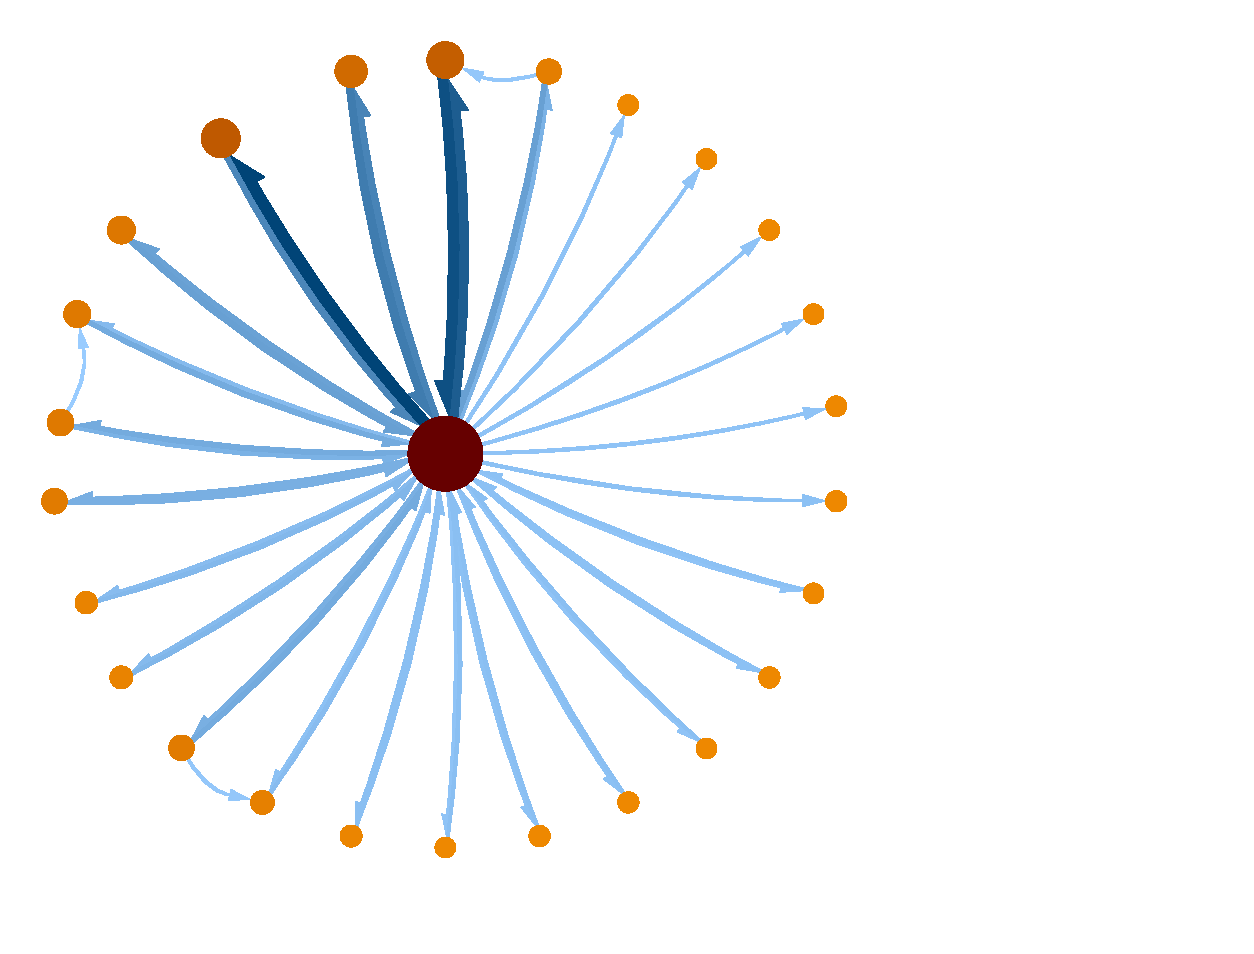
\includegraphics[width=0.4\linewidth]{ex-assortatividade-negativa.pdf}
        \label{fig:ex-assortatividade-negativa}
    }
    \subfloat[][Assortatividade $-0,07$] {
        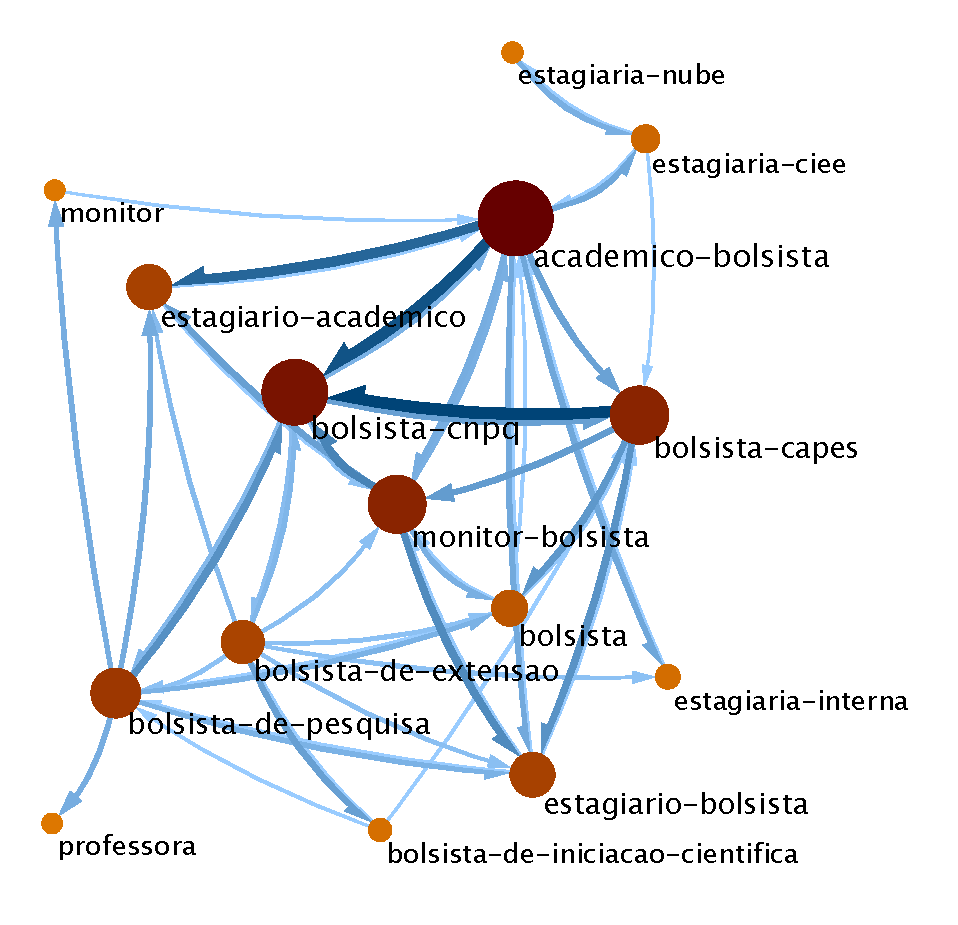
\includegraphics[width=0.4\linewidth]{ex-sobreposicao-bolsistas.pdf}
        \label{fig:ex-bolsistas}
    }    
    \caption{Assortatividade e Topologia}
\end{figure}

A assortatividade de grau em uma rede direcionada pode ser caracterizada pelo coeficiente de correlação de Pearson dos graus~\cite{Barabasi2016-rn}. Seja $k_i^\leftarrow$ e $k_i^\rightarrow$,  respectivamente, os graus de entrada e saída do nó $i$, seja $E$ o conjunto de conexões da rede, $e = (m, n) \mid e \in E$ as conexões de $E$, $m$ o vértice de onde $e$ sai e $n$ o vértice para onde $e$ aponta, definem-se os \textit{graus remanescentes} $\delta_e^\leftarrow$ e $\delta_e^\rightarrow$ da conexão $e$ como
\begin{align*}
\delta_e^\leftarrow &= k_n^\leftarrow - 1
\\
\delta_e^\rightarrow &= k_m^\rightarrow - 1\,.
\end{align*}

\begin{figure}[ht]
    \centering
    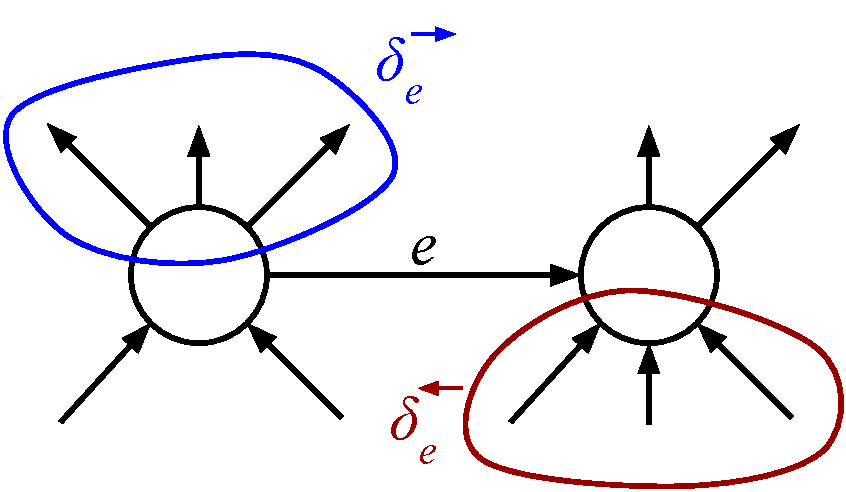
\includegraphics[scale=0.4]{remaining-degree.pdf}
    \caption{Graus remanescentes de entrada e saída da conexão $e$}
    \label{fig:remaining-degree}
\end{figure}

O \textit{grau remanescente} é o grau do nó, excetuando-se a conexão atual (Figura~\ref{fig:remaining-degree}). A correlação de Pearson $r$ dos graus é então definida por

\begin{align*}
p &= \sum_{e \in E} \delta_e^\leftarrow \delta_e^\rightarrow
\\
q &= \frac{1}{|E|} \sum_{e \in E} \delta_e^\leftarrow
                                  \sum_{e \in E }\delta_e^\rightarrow
\\
\sigma^2_\leftarrow &= \sum_{e \in E} \left( \delta_e^\leftarrow \right)^2
            - \frac{1}{|E|} \left( \sum_{e \in E} \delta_e^\leftarrow \right)^2
\\
\sigma^2_\rightarrow &= \sum_{e \in E} \left( \delta_e^\rightarrow \right)^2
           - \frac{1}{|E|} \left( \sum_{e \in E} \delta_e^\rightarrow \right)^2
\\
r &= \frac{p - q}
                {\sqrt{ \sigma^2_\leftarrow } \sqrt{ \sigma^2_\rightarrow }}\,.
\end{align*}


%===================================
\section{Resultados e Análises} \label{sec:resultados}
%===================================

% Descrição dos dados:

Os dados usadas para esse trabalho são do MCar de fevereiro de 2017. Após o processo de limpeza da informação o grafo resultante possui 7.267 nós e 145.115 conexões, sendo 68.771 bigramas e 76.344 trigramas.

A transformação dos bigramas e trigramas em conexões resulta em 73.064 conexões e essa versão é usada para caracterizar a rede quanto ao grau e conectividade.

A rede de ocupações possui a distribuição de grau exibida no gráfico de Pareto da Figura~\ref{fig:pareto-grau}. Ela possui uma grande concentração de conexões em poucos nós, formando \textit{hubs}. Os 25\% nós de maior grau são responsáveis por 85,86\% das conexões da rede.

Por ser uma rede direcionada, um certo cuidado na análise é necessário, uma vez que o grau dos nós não corresponde diretamente ao número de nós conectados. Imaginando que cada nó pode ter uma ou duas conexões com o mesmo nó vizinho, o grau $k_i$, varia em relação ao número de vizinhos entre $k_i = v_i$ (uma conexão por vizinho) e $k_i = 2v_i$ (cada vizinho possui uma conexão de entrada e saída com $k$), onde $v$ é o número de nós conectados ao nó $i$ por uma conexão de entrada ou saída.

A contribuição de cada nó para a conectividade da rede pode ser observada utilizando-se ego-grafos. Um ego-grafo é um subgrafo por um nó, todos os seus vizinhos e as conexões entre eles~\cite{Newman2010-od}. Como o número de conexões em uma rede direcionada não representa necessariamente o número de nós conectados, o uso do ego-grafo permite identificar \textit{hubs} que possuem maior conectividade sem que necessariamente possuam o maior número de conexões. Considerar o nó central junto aos seus vizinhos permite medir o quanto os subgrafos se sobrepõem sem a necessidade de ajustes quanto ao nó central.

No gráfico de Pareto da Figura~\ref{fig:pareto-egografo}. As ocupações estão ordenadas pelo tamanho do ego-grafo. Exatamente 25\% dos maiores ego-grafos são suficientes para conectar 98,31\% da rede. O nó de maior grau \textit{Auxiliar Administrativo} possui um ego grafo com 3.369 ocupações das da 7.267, ou seja, 46,36\% das ocupações de alguma forma possui fluxo de profissionais saindo ou entrando dessa ocupação.

A Tabela~\ref{tab:top-egografos} contém os 5 maiores ego grafos do MCar. Devido a presença de \textit{hubs} de grau elevado é esperado que os maiores ego-grafos compartilhem uma grande quantidade de nós.

\begin{table}[ht]
    \centering
    \begin{tabular}{@{} l r r r @{}}
    	\toprule
    	Ocupação                  & Ego-grafo & Acumulado & Inéditos \\
        \midrule
    	Auxiliar Administrativo   & 3.369    & 3.369     & 3.369    \\
    	Vendedor                  & 1.790    & 3.566     & 197      \\
    	Assistente Administrativo & 1.704    & 3.655     & 89       \\
    	Recepcionista                & 1.338    & 3.707     & 52       \\
    	Atendente                      & 1.249    & 3.739     & 32       \\
    	Auxiliar de Produção      & 1.061    & 3.954     & 215      \\
        \bottomrule
    \end{tabular}
    \caption{Tabela com os 5 maiores ego-grafos do MCar. A coluna \textit{Acumulado} contém o número de nós do ego-grafo da linha somado com os anteriores, excluindo-se nós já vistos. A coluna \textit{Inéditos} contém o número de nós que o ego-grafo possui que não estão nos ego-grafos anteriores.}
    \label{tab:top-egografos}
\end{table}

Essa característica reforça conceitos sobre movimentação profissional como a Carreira sem Fronteiras e a Carreira Proteana, indicando que uma grande quantidade de profissionais trilha por carreiras variadas e se adaptam a diferentes ocupações. No entanto, há uma rápida queda no número de conexões e no tamanho do ego-grafo, sugerindo que esses conceitos não se aplicam a todas as ocupações igualmente e que um número pequeno delas funciona como \enquote{coringa} ou \enquote{ponte} para movimentação profissional. Se essa característica está presente por que as ocupações são mais genéricas, por serem típicas do início de carreira ou por algum efeito de mercado é algo a ser investigado em trabalhos futuros.

%% Ronie: Aqui em cima tem algo que posso investigar na dissertação, acredito. Se há alguma correlação entre essas ocupações e escolaridade (sei que tem), e alguma correlação com o tempo de trabalho ou a idade.

O \enquote{Paradoxo da Amizade}~\cite{Barabasi2016-rn} parece valer para pessoas transitando entre ocupações. O paradoxo é dado como \enquote{na média, meus amigos são mais populares que eu}, transportado para o contexto desse trabalho seria enunciado como \enquote{na média, os outros trabalhos que eu poderia executar têm mais opções de movimentação que o meu}. Esse paradoxo tem uma explicação simples, como se observa na Figura~\ref{fig:pareto-egografo}, um nó qualquer têm grandes chances de estar conectado a um ou mais \textit{hubs} o que, na média, faz com que as ocupações vizinhas tenham mais conexões do que as suas próprias.

% Ronie: Esses dois parágrafos abaixo estão meio estranhos no texto. Mas os pontos são:
% 1 - Em uma rede direcionada, o ego-grafo é melhor de se analisar do que o grau. Isso pq, diferente de uma rede não-direcionada, o grau _não_ significa o número de vizinhos.
% 2 - Eu poderia ter usado um histograma (distribuição de frequência) para fazer uma análise similar. Na literatura de ciência de redes é praticamente o único gráfico que se vê. Mas, apesar das propriedades estatísticas interessantes, o histograma é bem menos informativo. O Pareto mostra claramente a contribuição dos hubs para a conectividade da rede, enquanto que o histograma relega eles a uma cauda fina e ruidosa (parece mais uma 'sujeira' do que a característica mais importante da rede). É um ponto que pode ser um pouco controverso (embora seja um detalhe), mas eu gostaria de tentar sustentá-lo melhor nesses parágrafos. Acha que vale o esforço ou é melhor 'passar reto' e nem mencionar?

A Figura~\ref{fig:pareto-egografo} ilustra a diferença entre o grau e a conectividade da rede que é importante do ponto de vista dessa pesquisa. Enquanto o grau identifica corretamente os \textit{hubs}, o gráfico de Pareto dos ego-grafos mostra que a rede é mais conectada do que seu número de conexões. Comparando os dois gráficos, percebe-se que, enquanto a distribuição de grau e do tamanho do ego-grafo são similares, o acumulado do primeiro cresce mais suavemente que o do segundo, indicando que os \textit{hubs} possuem proporcionalmente mais conexões unidirecionais, ou seja, menos conexões conectam mais nós.

Duas coisas a serem consideradas aqui, essa característica dos \textit{hubs} pode ser um efeito colateral do corte artificial de 5 conexões e uma análise similar poderia ser obtida projetando uma rede não-direcionada e analisando sua distribuição de grau.

\begin{figure}[htb]
  \centering
  \subfloat[][Pareto por Grau] {
    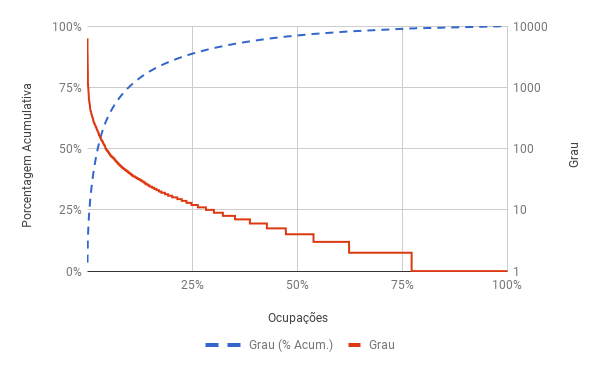
\includegraphics[width=0.49\linewidth]{pareto-grau}
    \label{fig:pareto-grau}
  }    
  \subfloat[][Pareto por Ego Grafo] {
      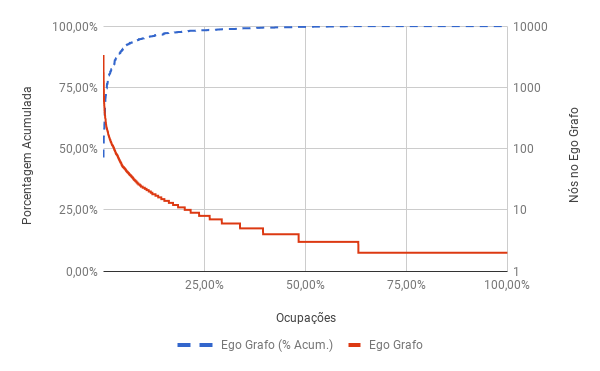
\includegraphics[width=0.49\linewidth]{pareto-egografo}
      \label{fig:pareto-egografo}
  }  
  \caption{Gráficos de Pareto com a distribuição de grau  do MCar e com o tamanho dos ego-grafos. Os gráficos estão colocados lado a lado para facilitar a comparação. Os nós estão ordenados de maneira decrescente no eixo horizontal; na Figura~\ref{fig:pareto-grau}  as ocupações de grau maior no estão à esquerda e ocupações de menor grau estão à direita. na Figura~\ref{fig:pareto-egografo} elas estão ordenadas pelo tamanho do ego-grafo. Os eixos direitos, em escala logarítmica, estão associados às linhas cheias e representam, respectivamente, o grau do nó e o tamanho do ego-grafo. Os eixos esquerdos estão associados às linhas tracejadas; na Figura~\ref{fig:pareto-grau} ela representa a somatória de todos os graus em porcentagem e qual a contribuição das ocupações à esquerda para essa totalização; na Figura~\ref{fig:pareto-egografo} ela representa a quantidade de ocupações que os ego-grafos à esquerda conectam.}
  \label{fig:paretos}
\end{figure}

Observando a Figura~\ref{fig:paretos} é possível notar que cerca de $1/5$ das ocupações possui apenas uma conexão (1.547 delas, 21,29\%), mas pouco mais de $1/3$ (2.682 delas, 36,91\%) possui um ego-grafo de tamanho 2. A diferença entre ambos são os ego-grafos que possuem múltiplas conexões, tanto auto-referentes quanto de entrada e saída com seu vizinho.

Isso indica que grande parte das ocupações ($1/3$) está na \enquote{borda} da rede, conectada a ela por apenas um vizinho. Se os \textit{hubs} reforçam os conceitos de Carreiras Proteanas e Carreiras sem Fronteiras, a quantidade de ocupações na borda da rede indica o contrário. A presença de ambas as características sugere novamente que as teorias mencionadas não se aplicam a todas as ocupações. Apesar dessa pesquisa conseguir indicar quais ocupações parecem se encaixar melhor nessas teorias e quais não, ela é incapaz de responder quais são as alternativas e por que elas acontecem.

% Ronie: O parágrafo acima me parece um ótimo gancho para alguém que trabalhe com essa parte. Gostaria de deixar isso bem atraente :D (mas não sei se cabe).

Nos experimentos realizados, o algoritmo Infomap foi utilizado para encontrar o particionamento mais coeso do MCar em relação ao fluxo. Como exposto nas Seções~\ref{sec:carreira} e~\ref{sec:infomap}, esse particionamento é a própria definição de fronteiras de carreira.

\begin{comment}
Ronie: Vou tirar isso aqui, levanta mais dúvidas do que esclarece e em (quase) nenhum artigo que li eles explicam quais parâmetros foram utilizados. Entendo que facilita a reprodutibilidade, mas acho melhor eu tentar trabalhar em disponibilizar os dados =)

====

O Infomap é bastante robusto quanto aos parâmetros utilizados, ou seja, mesmo grandes variações em seus parâmetros devem produzir resultados similares~\cite{Kawamoto2015-ha,Lambiotte2012-fp}. Por essa razão foi usado o parâmetro padrão de probabilidade de teleporte de 0,15.
\end{comment}

Para esse algoritmo, quanto maior a compressão da informação do caminho do \textit{random walker}, melhor é o particionamento da rede~\cite{Rosvall2009-sd}.

O MCar foi testado em duas variações do algoritmo: 
\begin{itemize}
\item Simples: consiste na detecção de comunidades em que cada nó pertence a apenas uma única comunidade. 
\item Com sobreposição: permite-se que nós participem de mais de uma comunidade.
\end{itemize}

A variação com maior compressão revela a melhor caracterização de particionamento~\cite{Viamontes_Esquivel2011-it,Rosvall2011-yi,Edler2017-kt}. Se a variação com sobreposição possuir maior compressão de informação do que as outras, assume-se que suas comunidades, intrinsecamente, compartilham nós.

Os resultados de compressão para cada variação são apresentados na Tabela~\ref{tab:metodos}. É possível observar que há ganho na compressão de informação quando se permite a sobreposição de comunidades, revelando a movimentação dos profissionais é melhor caracterizada quando as ilhas compartilham ocupações. Uma quantidade relativamente pequena de ocupações,  cerca de 11\%, é compartilhada entre ilhas.

% INTUITIVAMENTE UMA COMPRESSÃO MAIOR IMPLICA EM MENOS COMUNIDADES, PORÉM SUA TABELA MOSTRA O CONTRÁRIO, ASSIM COMO O TEXTO. DE ACORDO COM SUA EXPLICAÇÃO UMA MAIOR COMPRESSÃO IMPLICA EM MELHOR PARTICIONAMENTO E, PORTANTO, MAIS COMUNIDADES.
% Ronie: Aqui acho que preciso melhorar a explicação. Como tb não expliquei as variações hierárquicas e com sobreposição do Infomap estão também falta uma peça do quebra cabeças. A compressão dessa 'descrição do caminho do random walker' acaba criando um balanço entre quantidade de nós e de comunidades. Se não houverem 'gargalos' de fluxo, o random walker não fica 'preso' em um subgrafo e a melhor compressão acontece simplesmente por códigos mais curtos nos nós mais frequentes, sem divisão em comunidades. Por outro lado, quando existe um gargalo o random walker fica preso por um longo tempo de um lado ou de outro dele, nesse formato a melhor compressão acontece se cada 'prisão' reutilizar os códigos mais curtos e criarmos um outro código para passar de um lado para o outro do gargalo. O que está acontecendo na variação com sobreposição é que existem nós, ao invés de conexãos, que são fronteira entre as comunidades. Uma boa ilustração disso é o grafo 'gravata borboleta' com 5 nós e 6 conexões, nesse formato: ▷◁. Sem permitir sobreposição de comunidades, o nós central força os dois triângulos a pertencer em uma única comunidade. Permitindo a sobreposição, o nó central consegue participar de duas comunidades: ▷ e ◁. Se fosse uma rede com uma conexão entre os triângulos, desse jeito: ▷—◁, então o gargalo seria a conexão (não o nó) e o algoritmo que não permite sobreposição teria a melhor compressão.

\begin{table}
  \centering
  \begin{tabular}{@{} l r r @{}}
  	\toprule
  	Variação         & Compressão & Ilhas Ocupacionais \\
    \midrule
  	Simples          & 46,08\%    & 65                \\
  	Com sobreposição & 50,30\%    & 624                \\
    \bottomrule
  \end{tabular}
  \caption{Métodos de detecção de comunidades e seus resultados. O \textit{Método} se refere ao tipo (variação) de particionamento. \textit{Compressão} significa qual a compressão de informação obtida pelo Infomap em relação a uma rede sem particionamento. \textit{Ihas Ocupacionais} é o número de partições não-triviais resultantes (ao menos 3 nós na comunidade).}
  \label{tab:metodos}
\end{table}

Apesar de usar a expressão \enquote{compartilham ocupações}, a interpretação mais correta é que as ilhas possuem \textit{suas próprias versões} das ocupações. \citeonline{Viamontes_Esquivel2011-it} apresentam um exemplo intuitivo do significado desse \enquote{compartilhamento} usando aeroportos europeus e norte-americanos. Transposto para a realidade do MCar, uma ocupação que pertence a mais de uma comunidade significa que os profissionais que transitam por ela, em sua maioria, voltam aos seus grupos de origem ao invés de migrarem para outros. Não fosse dessa forma, esses grupos conectados seriam considerados como um conjunto único de ocupações pelo algoritmo ou a ocupação estaria em apenas na comunidade com fluxo predominante.

Existem duas explicações possíveis. A primeira é que essas ocupações são \textit{homônimas} e, portanto, distintas, o que significa que há uma fronteira entre elas. A segunda é que essas ocupações são similares, mas fatores não especificados dificultam a transição de um grupo para outro, o que também indica uma fronteira de carreira, ainda que mais fraca.

Um exemplo da primeira explicação é a ocupação \enquote{Coordenador de Projetos}, que está associada tanto à Arquitetura quanto à Software. Um possível exemplo da segunda é a ocupação de \enquote{Professor} que aparece em diversas ilhas, sugerindo que há especializações nessa ocupação que impedem que um Professor se movimente entre ilhas, o que condiz com o conhecimento tácito sobre a profissão, um Professor de Matemática não se transforma em um Professor de Língua Portuguesa facilmente.

Em qualquer uma dessas interpretações, as ocupações que participam de mais de uma ilha ocupacional revelam uma fronteira e não uma ponte.

\begin{comment}
Ronie: Lá se vai mais um pedaço do trabalho pro brejo :D Lição aprendida: o trabalho de pesquisa tem muito 'vai e vem', não compensa escrever coisas em detalhes e caprichar no português até a trabalho estar quase concluído. O próximo vai funcionar melhor e ser bem mais rápido :)

====

Os resultados obtidos foram comparados com o trabalho de \citeonline{Viamontes_Esquivel2011-it} para obter uma perspectiva mais ampla sobre o significado da compressão (Tabela~\ref{tab:comparativo}). É possível observar que o MCar é a rede que mais se beneficia de uma estrutura que permite sobreposição de comunidades.

\begin{table}
  \centering
  \begin{tabular}{@{} l r r r r r @{}}
    \toprule
                                           &      &          & \multicolumn{2}{c}{Compressão} & \\
    \cmidrule(r){4-5}
    Rede                                   & Nós  & Conexões & Simples & $\Delta$ Sobr.       & $N_{\text{sobr}}/N$ \\
    \midrule
    \rowcolor{yellow!25} Mapa de Carreiras & 7450 & 90800    & 14\%    & 30\%                 & 11\% \\
    Estradas Europeias                     & 1018 & 1274     & 46,2\%    & 10,4\%                 & 35,5\% \\
    Grade de Energia Leste dos EUA         & 4941 & 6994     & 53,4\%    & 8,8\%                  & 27,5\% \\
    Doenças Humanas                        & 516  & 1188     & 46,4\%    & 2,9\%                  & 15,3\% \\
    Coautoria de Artigos de Ciência de Redes                   & 552  & 1317     & 48,9\%    & 2,5\%                  & 14,6\% \\
    Rotas Aéreas                           & 3618 & 14142    & 31,1\%    & 1,2\%                  & 13,9\% \\
    Blogs Políticos (EUA)                  & 1222 & 16714    & 4,1\%     & 0,4\%                & 5,8\% \\
    Blogs Políticos (Suécia)               & 855  & 10315    & 0,5\%   & 0,2\%                & 4,8\% \\
    Rede Neural \textit{C. elegans}        & 297  & 2345     & 1,7\%     & 0,1\%                & 2,7\% \\
    \bottomrule
  \end{tabular}
  \caption{Comparativo da estrutura do Mapa de Carreiras (em destaque) com outras redes~\cite{Viamontes_Esquivel2011-it}. \textit{Compressão Simples} se refere à compressão de informação onde o Infomap obteve o melhor particionamento simples da rede (sem sobreposição ou hierarquia de partições). \textit{Compressão $\Delta$ Sobr.} se refere ao ganho na compressão obtido pela sobreposição de partições em relação à compressão simples. $N_{\text{sobr}}/N$ é a proporção de nós que participam em mais de uma comunidade em relação ao total de nós.}
  \label{tab:comparativo}
\end{table}

A distribuição de tamanho das ilhas resultantes da partição com sobreposição está na Figura~\ref{fig:pareto-comunidades}. Mais de 75\% delas possui uma única ocupação, representando apenas 8\% de todas as ocupações. 
\end{comment}

\begin{figure}[htb]
    \centering
    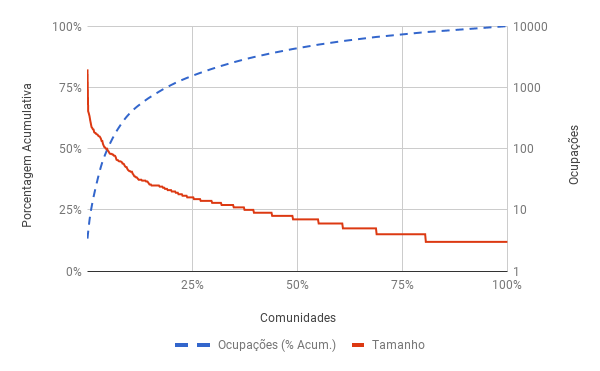
\includegraphics[width=0.9\linewidth]{pareto-comunidades.png}
    \caption{Gráfico de Pareto com a distribuição de tamanho das ilhas ocupacionais. As comunidades estão ordenadas pelo número de ocupações que contêm, ilhas maiores estão à esquerda e menores à direita. O eixo direito, em escala logarítmica, está associado à linha cheia e representa o número de ocupações da ilha. O eixo esquerdo está associado à linha tracejada e representa o total de ocupações e qual a contribuição acumulativa das ilhas à esquerda do ponto para ela.}
    \label{fig:pareto-comunidades}
\end{figure}

As comunidades, em sua maioria, possuem uma topologia em que predomina a forma de estrela ou estrelas com múltiplos centros. Isso significa poucos \textit{hubs} conectando quase todos os outros nós. Esse formato é caracterizado por uma assortatividade negativa, ou seja, nós de alto grau conectados a nós de baixo grau~\cite{Barabasi2016-rn}.

A assortatividade das 624 ilhas com ao menos três ocupações é exibida na Figura~\ref{fig:assortatividade}. Quase todas elas possuem assortatividade negativa, confirmando a existência de polos ocupacionais. Na Figura~\ref{fig:ex-ilhas-ocupacionais} são apresentados três exemplos emblemáticos sobre a assortatividade e o efeito esperados dos polos.

\begin{figure}[htb]
    \centering
    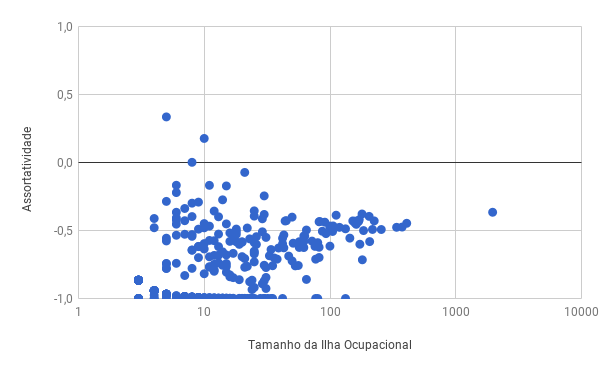
\includegraphics[width=0.9\linewidth]{assortatividade.png}
    \caption{Assortatividade pelo número de ocupações na ilha com o eixo $x$ em escala logarítmica.}
    \label{fig:assortatividade}
\end{figure}

A ilha que se inicia com \enquote{Aluno de Iniciação Científica} é exibida na Figura~\ref{fig:ex-sobreposicao-ciencia}. A topologia estrelada é claramente observável, irradiando-se a partir do \textit{polo ocupacional}. O fluxo predominante parte de \textit{Aluno de Iniciação Científica}, passa por \textit{Aluno de Mestrado} e termina em \textit{Aluno de Doutorado} sem que haja fluxo na direção contrária, reforçando o conhecimento tácito sobre a área.

O polo ocupacional é claramente \textit{Aluno de Iniciação Científica}. O reforço dessa ocupação deve distribuir o fluxo de pessoas para as outras ocupações, em especial o fluxo mais forte \textit{Aluno de Mestrado} $\rightarrow$ \textit{Aluno de Doutorado}. Por outro lado, seu enfraquecimento tende a minar o fluxo de pessoa para outras ocupações, provocando o enfraquecimento da ilha como um todo.

Essa análise pontual dá dimensão à contribuição desse trabalho. Nesse caso, identificada a ilha, o polo e o fluxo predominante,  ações para reforçar uma ocupação, como \textit{Aluno de Doutorado}, por exemplo, passam a ser óbvias. Essa análise superficial sugere que aumentar o número de alunos de iniciação científica, desestimular sua movimentação para outras ocupações ou incentivar o fluxo para o mestrado provocaria o efeito desejado. A proporção de pessoas em cada fluxo fornece um \enquote{funil} para se estimar quantas pessoas seriam necessárias em cada ocupação para atingir um certo resultado.

As proporções entre as ocupações, por exemplo, entre \textit{Aluno de Iniciação Científica}, \textit{Aluno de Mestrado} e \textit{Aluno de Doutorado} também podem servir como comparativo entre uma instituição de ensino e o \enquote{mercado}.

A ilha ocupacional relacionada à \textit{Tecnologia da Informação}, exibida na Figura~\ref{fig:ex-sobreposicao-ti}, possui uma topologia de estrela com três polos claros: \textit{Gerente de Projetos}, \textit{Analista de Sistemas} e \textit{Analista de Suporte}. Cada um deles funciona como centro de seu próprio conjunto de ocupações, mas com grande movimentação de profissionais entre si.

A remoção de um desses polos desconectaria a parte das ocupações em que esse polos são a única conexão com a ilha ocupacional, mas não seria suficiente para esfacelá-la como no caso anterior. A conexão de maior fluxo nessa ilha está entre \textit{Analista de Suporte} $\rightarrow$ \textit{Analista de Sistemas}. Chama a atenção não haver um fluxo direto significativo entre \textit{Analista de Suporte} e \textit{Gerente de Projetos}, indicando que \textit{Analista de Sistemas} pode funcionar como uma \textit{ponte} entre essas ocupações.

%% EXISTE UM DESEQUILÍBRIO NA PROFUNDIDADE DA EXPLICAÇÃO DO CASO 1 PARA ESTE CASO 2 E O PRÓXIMO, FAVOR BALANCEAR.
% Ronie: Feito, mas não consegui aprofundar mais.

No último exemplo da Figura~\ref{fig:ex-sobreposicao-vendas}, exibindo a ilha relacionada a \textit{Comercial e Vendas}, os polos não são tão claros. \textit{Gerente Comercial} e \textit{Consultor de Vendas} se destacam, mas quatro outros nós possuem grande fluxo e alta conectividade. A remoção de um desses nós não afetaria a rede da mesma forma que nos exemplos anteriores. Nota-se também que há um forte fluxo entre todos os nós de maior fluxo, diferentemente do exemplo da ilha de \textit{Tecnologia da Informação}, em que dois dos polos possuem conexão tão tênue que não figura entre as conexões de maior fluxo da rede.

A topologia é mais similar a de \textit{centro e raios}, em que as ocupações mais periféricas se conectam entre si, mas ainda assim possuem um grau elevado de conexões.

\begin{figure}[ht]
    \centering
    \subfloat[][Iniciação Científica] {
        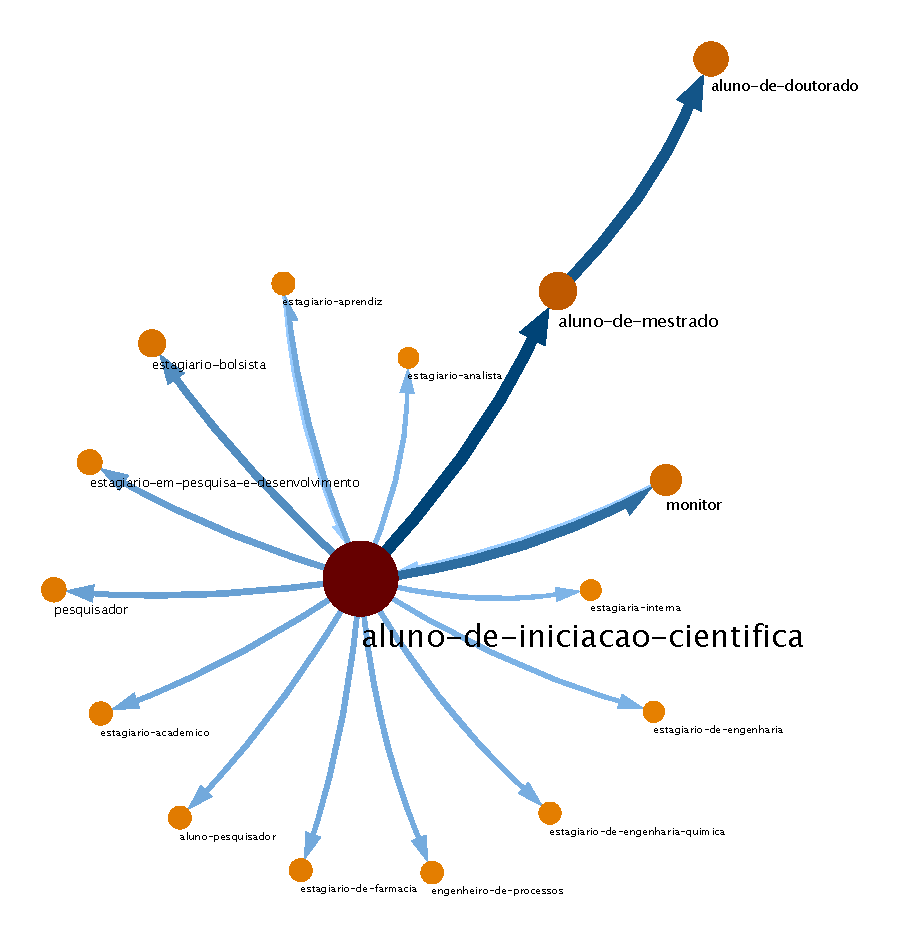
\includegraphics[width=0.5\linewidth]{ex-sobreposicao-aluno-iniciacao.pdf}
        \label{fig:ex-sobreposicao-ciencia}
    }
    \subfloat[][Tecnologia da Informação] {
        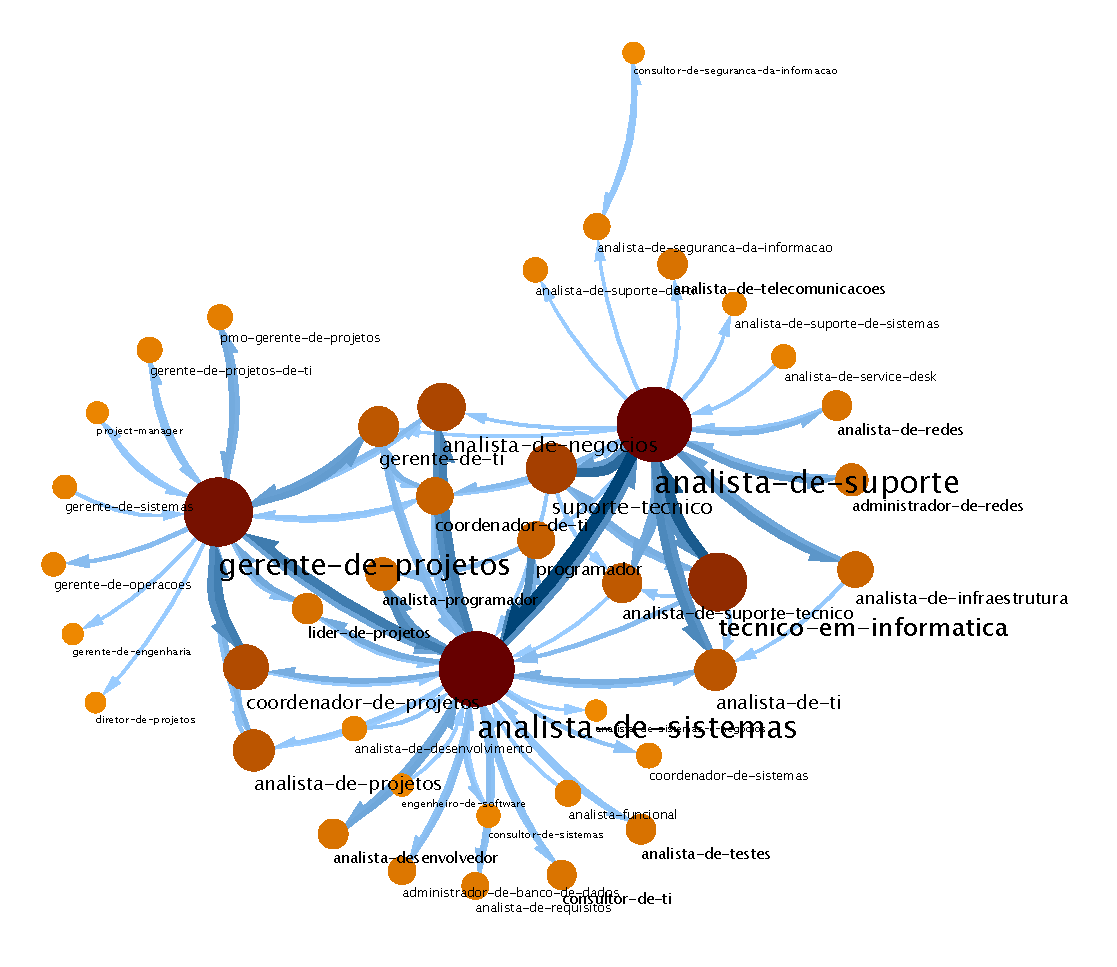
\includegraphics[width=0.5\linewidth]{ex-sobreposicao-analista-de-sistemas.pdf}
        \label{fig:ex-sobreposicao-ti}
    }
    \\    
    \subfloat[][Comercial e Vendas] {
        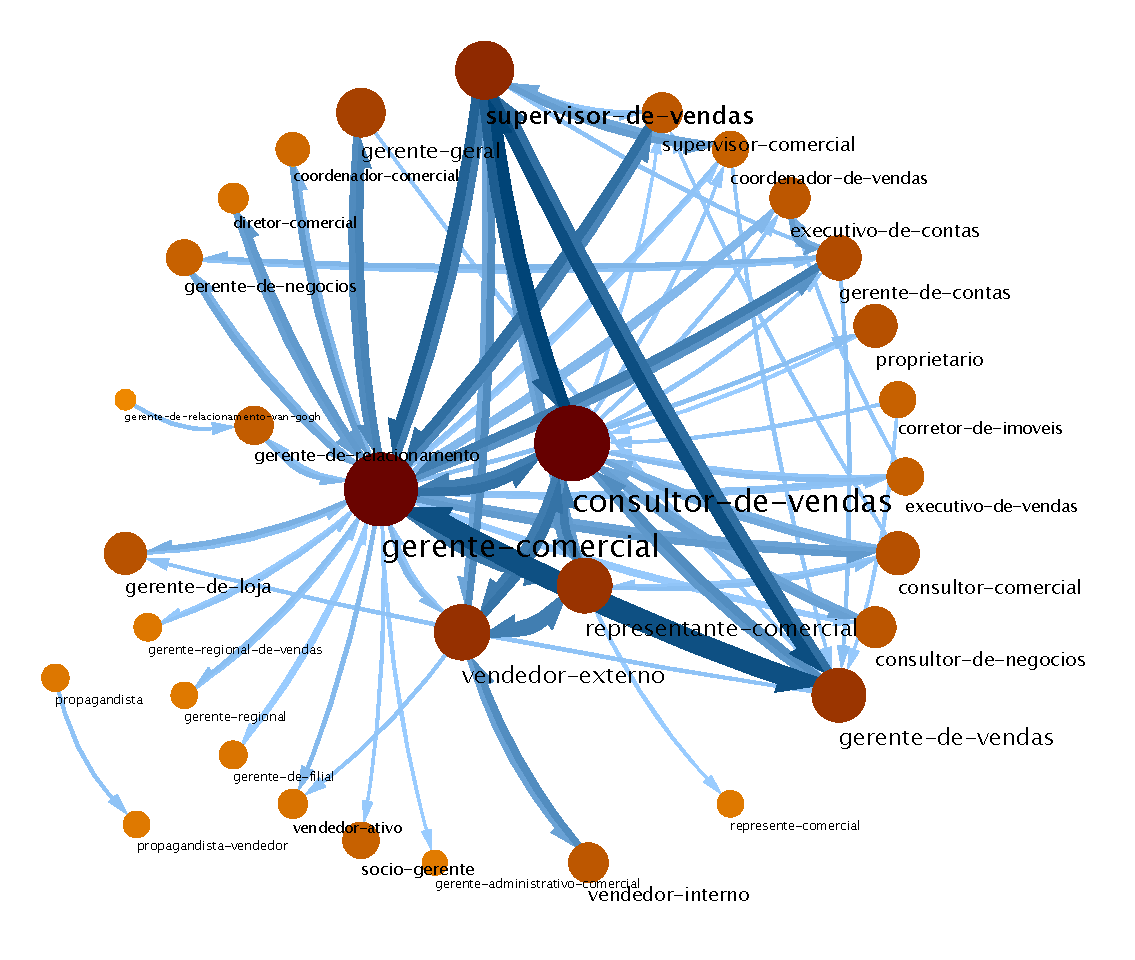
\includegraphics[width=0.5\linewidth]{ex-sobreposicao-consultor-de-vendas.pdf}
        \label{fig:ex-sobreposicao-vendas}
    }
    \caption{Três exemplos de ilhas ocupacionais. O tamanho e a cor do nó estão relacionados ao fluxo de profissionais que passa por ele, quanto maior e mais escuro o nó, maior o fluxo. Da mesma forma, a espessura e a cor das conexões está relacionada ao fluxo de profissionais entre uma ocupação e outra. O polos ocupacionais são identificados pelo volume de pessoas transitando por eles e pela sua alta conectividade (visualmente os nós maiores e mais centrais). Para facilitar a visualização, nas Figuras~\ref{fig:ex-sobreposicao-ti} e~\ref{fig:ex-sobreposicao-vendas}, apenas as conexões e nós de maior fluxo são apresentados. A Figura~\ref{fig:ex-sobreposicao-ciencia}, no entanto, mostra a ilha completa.}
    \label{fig:ex-ilhas-ocupacionais}
\end{figure}

%===================================
\section{Conclusões e Perspectivas Futuras}
%===================================

Esse trabalho reúne os conceitos fronteiras de carreira de \citeonline{Gunz2007-hr}, os trabalhos de Ciência de Redes sobre detecção de comunidades por fluxo baseados em \cite{Rosvall2009-sd} e os dados de um dos maiores sites brasileiros de carreira~\cite{VAGAS_Tecnologia2014-yv} para contribuir na compreensão da movimentação profissional.

A rede profissional possui \textit{hubs}, o que fornece indícios de que carreiras menos regulares são comuns, como advogam as Carreiras sem Fronteiras e Carreiras Proteanas. Ao mesmo tempo a presença de muitos pequenos ego-grafos e ilhas ocupacionais diminutas sugerem que há alternativas para essas teorias.

O algoritmo Infomap foi aplicado para identificar as fronteiras de carreiras, gerando \textit{ilhas ocupacionais}, que são conjuntos de ocupações em que a movimentação interna é significativamente mais frequente do que movimentações para outras \textit{ilhas}. O termo foi introduzido para facilitar a discussão e como uma analogia ao conceito sugerido por~\cite{Abbott1995-ft} em que a fronteira define o grupo, ao invés do grupo definir a fronteira. Essa abordagem usa a diferença entre os grupos para defini-los ao invés de alguma característica intrínseca. 

A análise da assortatividade das ilhas mostrou que sua topologia tende ao formato estrelado ou de eixo e raios, o que motivou a introdução do termo \textit{polos ocupacionais} para identificar ocupações que dão coesão à ilha. Alguns exemplos emblemáticos dão dimensão aos dois conceitos introduzidos nesse trabalho.

Conclui-se na expectativa que esse trabalho contribua para na compreensão das transições profissionais, no entanto, é preciso reconhecer as limitações dessa proposta e as questões que permanecem abertas.

Os aspectos sociais e psicológicos das fronteiras de carreira não foram abordados e são eles quem podem responder a perguntas como \enquote{por que as fronteiras estão onde estão?} e \enquote{por que as ilhas possuem essa topologia?}. Espera-se que o conteúdo apresentado contribua de maneira quantitativa em discussões sociais e psicológicas sobre movimentação profissional.

Outros trabalhos podem aprofundar a questão da dinâmica da rede, focando em modelos que possam predizer os efeitos esperados quando uma ocupação ganha ou perde atratividade, ou quando um fluxo é incentivado ou estrangulado. Esse trabalho ensaia um começo tímido nessa direção ao propor o conceito de polos ocupacionais e identificar sua importância nas ilhas de ocupações.

Outra linha de pesquisa atrativa está em comparar o MCar com redes aleatórias geradas a partir de características similares à da rede real, procurando identificar quais delas resultam em observações comparáveis. Essas características indicam possíveis explicações para os comportamentos encontrados a partir de uma abordagem puramente estatística~\cite{Barabasi2016-rn}.

O MCar é uma fonte considerável de informação sobre o mercado de trabalho brasileiro. Outras pesquisas sobre profissões e carreira, em especial utilizando técnicas de Ciência de Redes, como \textit{motifs}, podem contribuir para uma melhor compreensão da movimentação profissional.

\newpage

\bibliography{main}
\end{document}
